% Chapter Template

\chapter{Results and Discussion} % Main chapter title

\label{c5} % Change X to a consecutive number; for referencing this chapter elsewhere, use \ref{ChapterX}


% \section{Results and Discussion}\label{sec2}
In this paper, the Upward batch and Downward batch ensemble(UD-Batch) are used. In the UD-Batch ensemble, first, we shifted the dataset $n$ times upward and $n$ times downward with the same step value. Then, we applied traditional DL models on upper shifted datasets and ensemble the predictions similarly done for downward shifted datasets to get the downward prediction, and at last, we ensemble the upward prediction and downward prediction. There is also a second approach called Corresponding upward and downward ensemble(CUD-ensemble) in which we ensemble the individual upshifted and downshifted predictions and then take an average of all individual predictions. In Fig. \ref{fig:all_models_mae}, Fig.\ref{fig:all_models_rmse}, Fig.\ref{fig:all_models_mse}, Fig.\ref{fig:all_models_mape} dark area showing the MAE, RMSE, MSE, MAPE of UD-Batch ensemble respectively and light area showing the MAE, RMSE, MSE, MAPE of UD-Batch ensemble respectively so here clearly shown that UD-Batch ensemble more precise then CUD-ensemble. The overall conclusion is that the ensemble technique has been used in this research among the two proposed ensemble techniques, UD-Batch.
\begin{figure}[ht!]
%\centering
\subfloat[LSTM: UD-Batch ensemble Vs CUD ensemble]{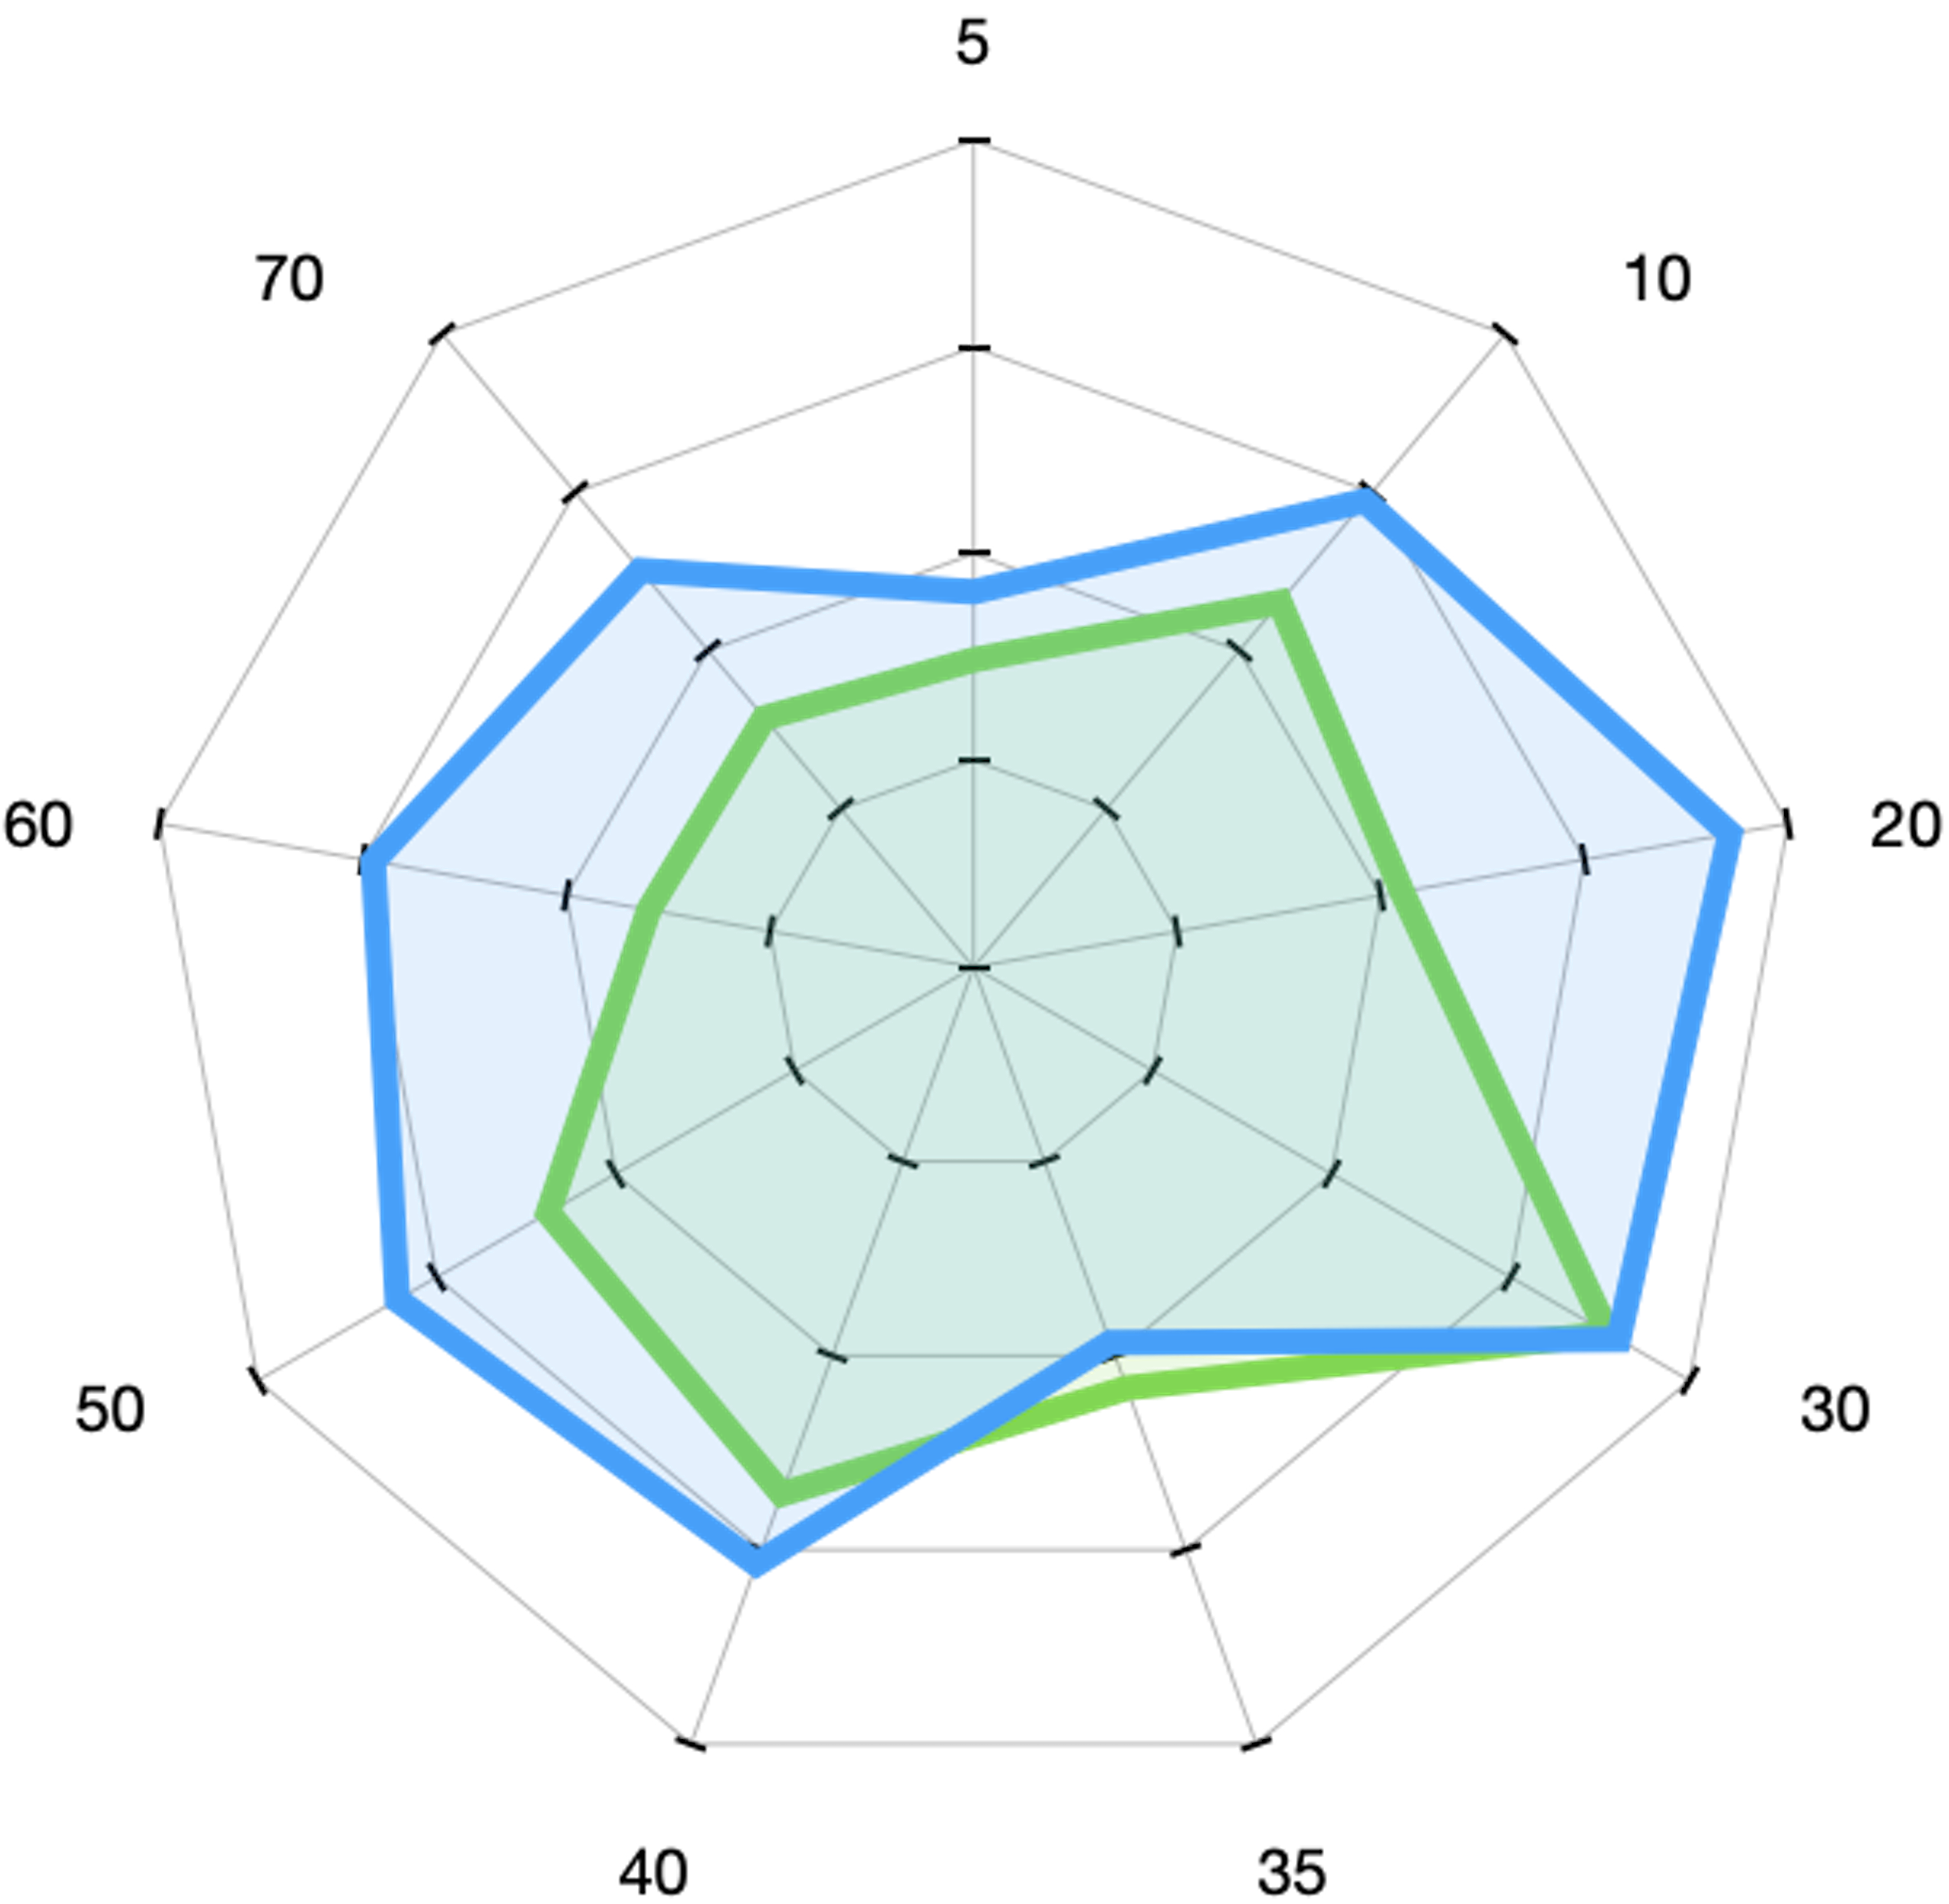
\includegraphics[width=0.4\textwidth, height=0.3\linewidth]{LSTM_MAE_SPIDER.png}\label{fig:LSTM MAE SPIDER}}
\hfill
\subfloat[RNN: UD-Batch ensemble Vs CUD ensemble]{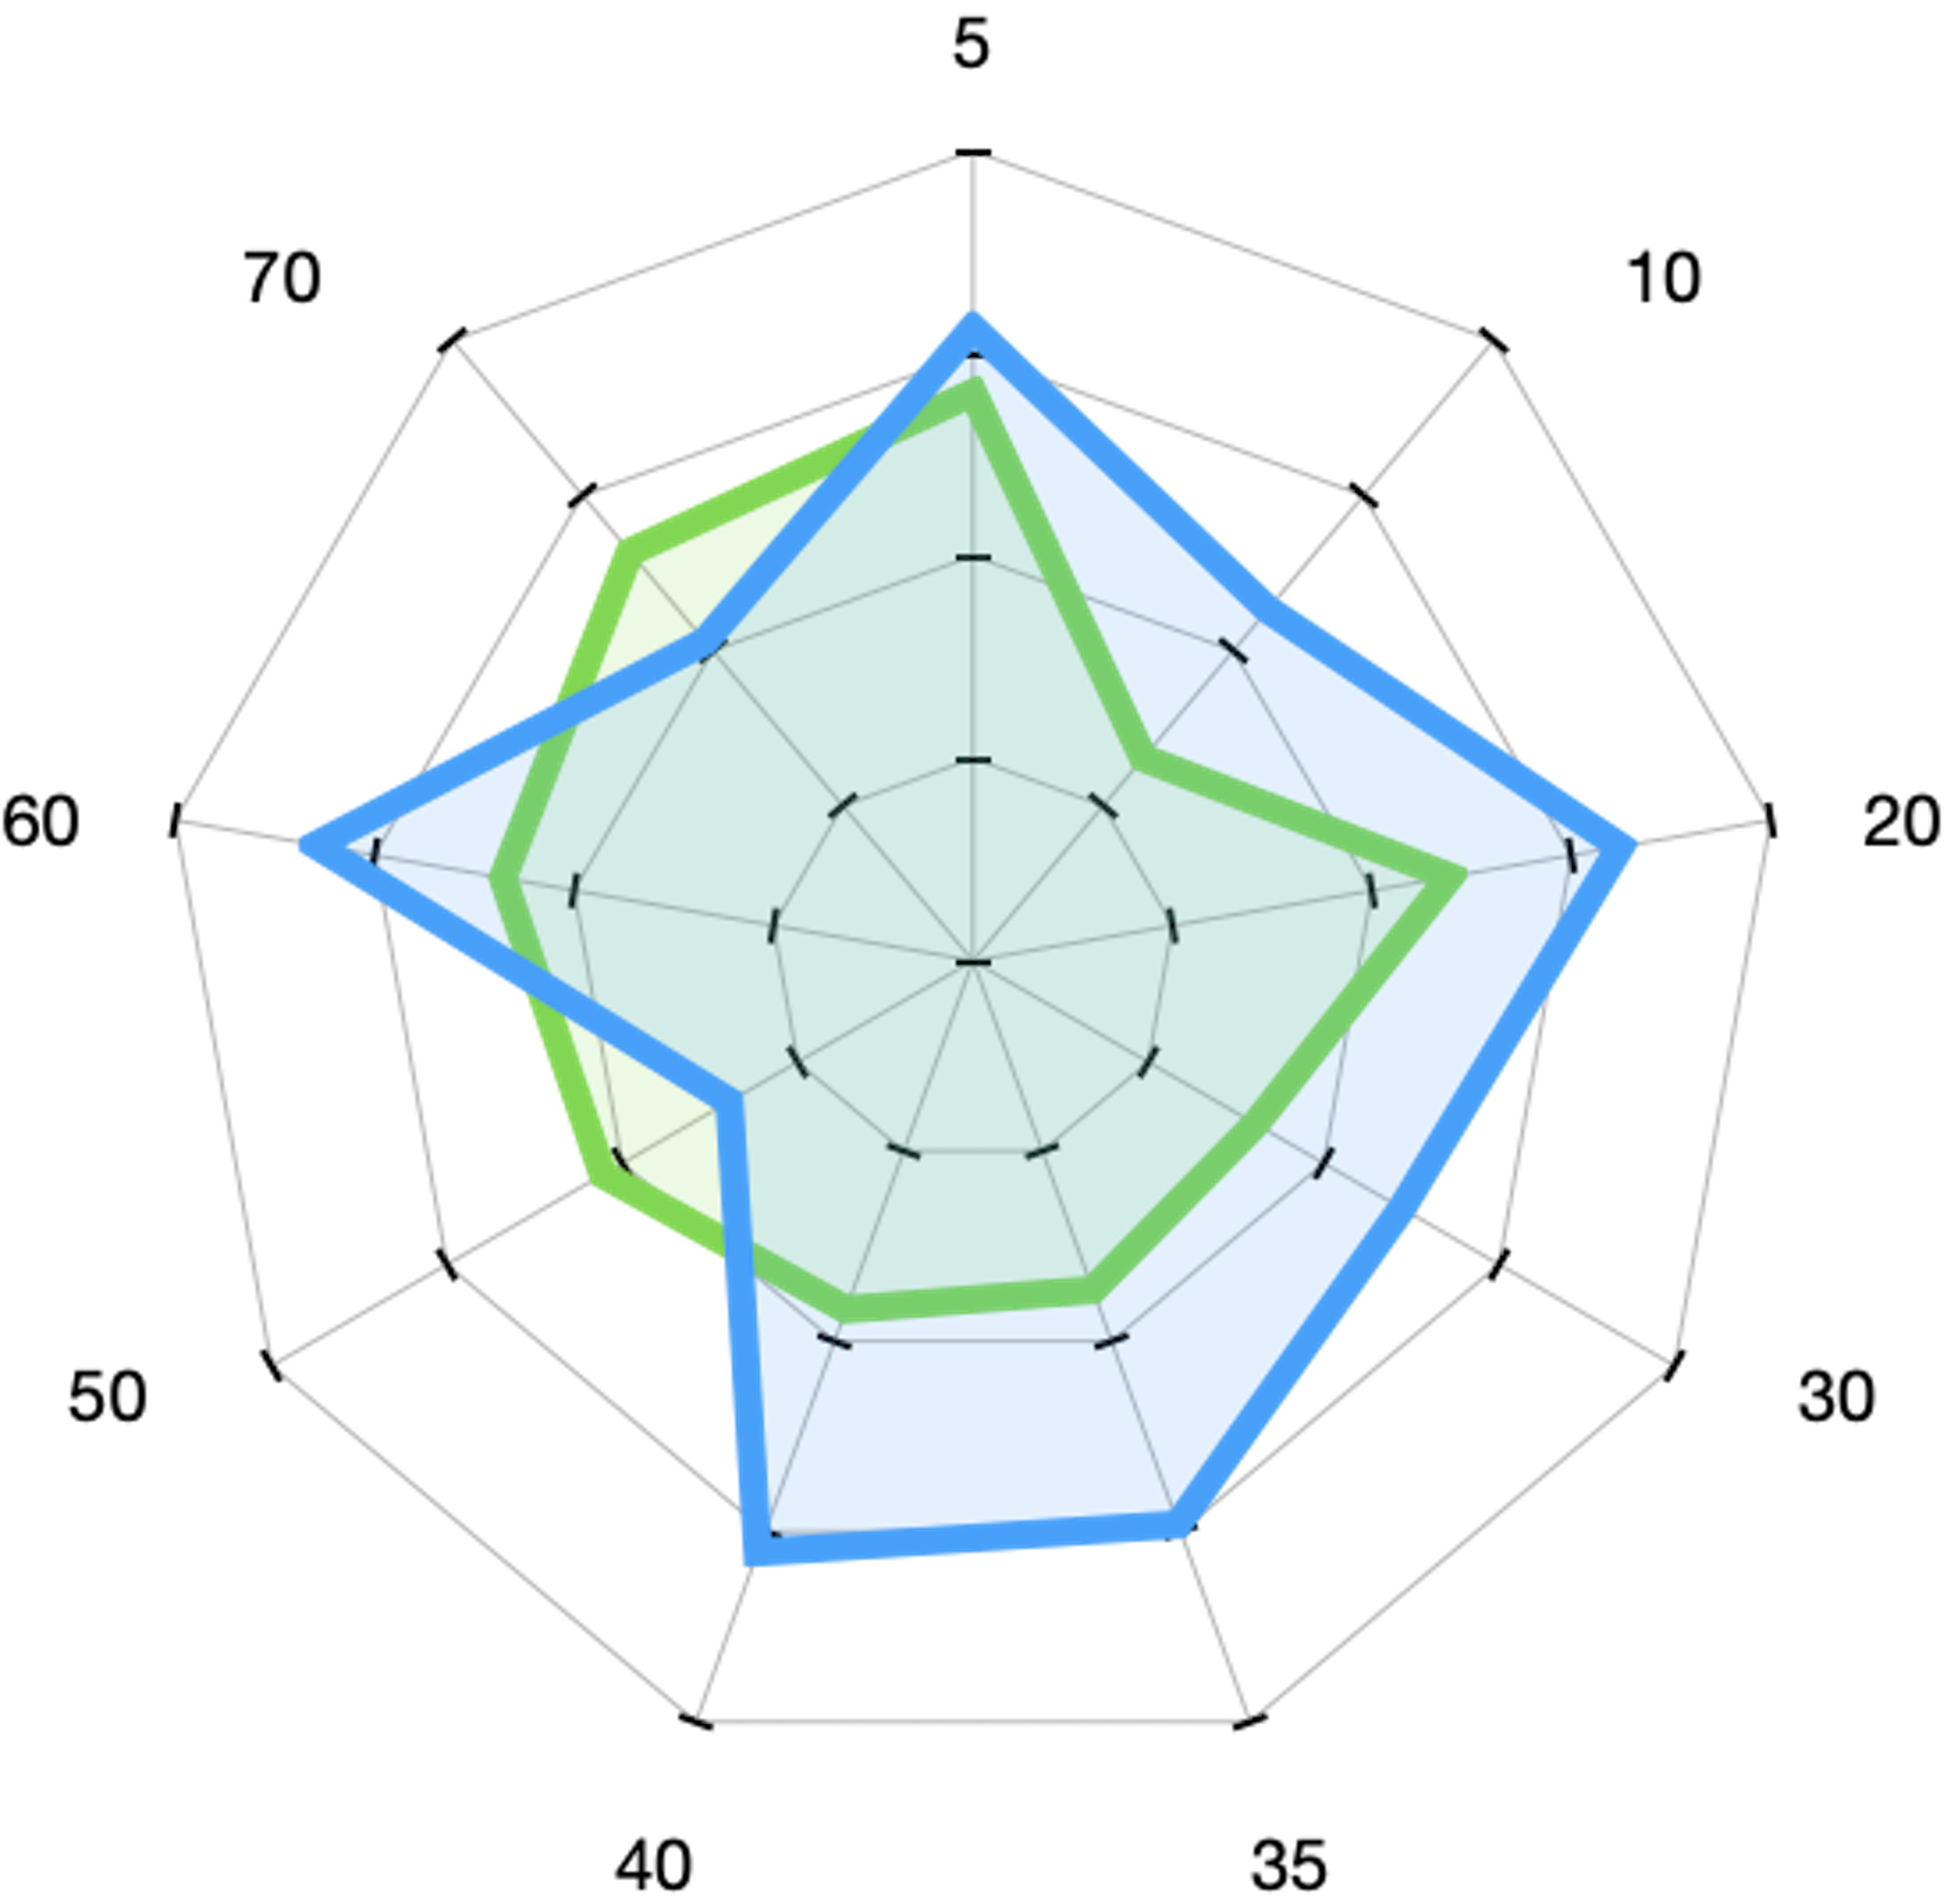
\includegraphics[width=0.4\textwidth, height=0.3\linewidth]{RNN_MAE_SPIDER.png}\label{fig:RNN_MAE_SPIDER}}\\
\subfloat[BiLSTM: UD-Batch ensemble Vs CUD ensemble]{\includegraphics[width=0.4\textwidth, height=0.3\linewidth]{Bi-LSTM_MAE_SPIDER.png}\label{fig:BiLSTM_MAE_SPIDER}}
\hfill
\subfloat[GRU: UD-Batch ensemble Vs CUD ensemble]{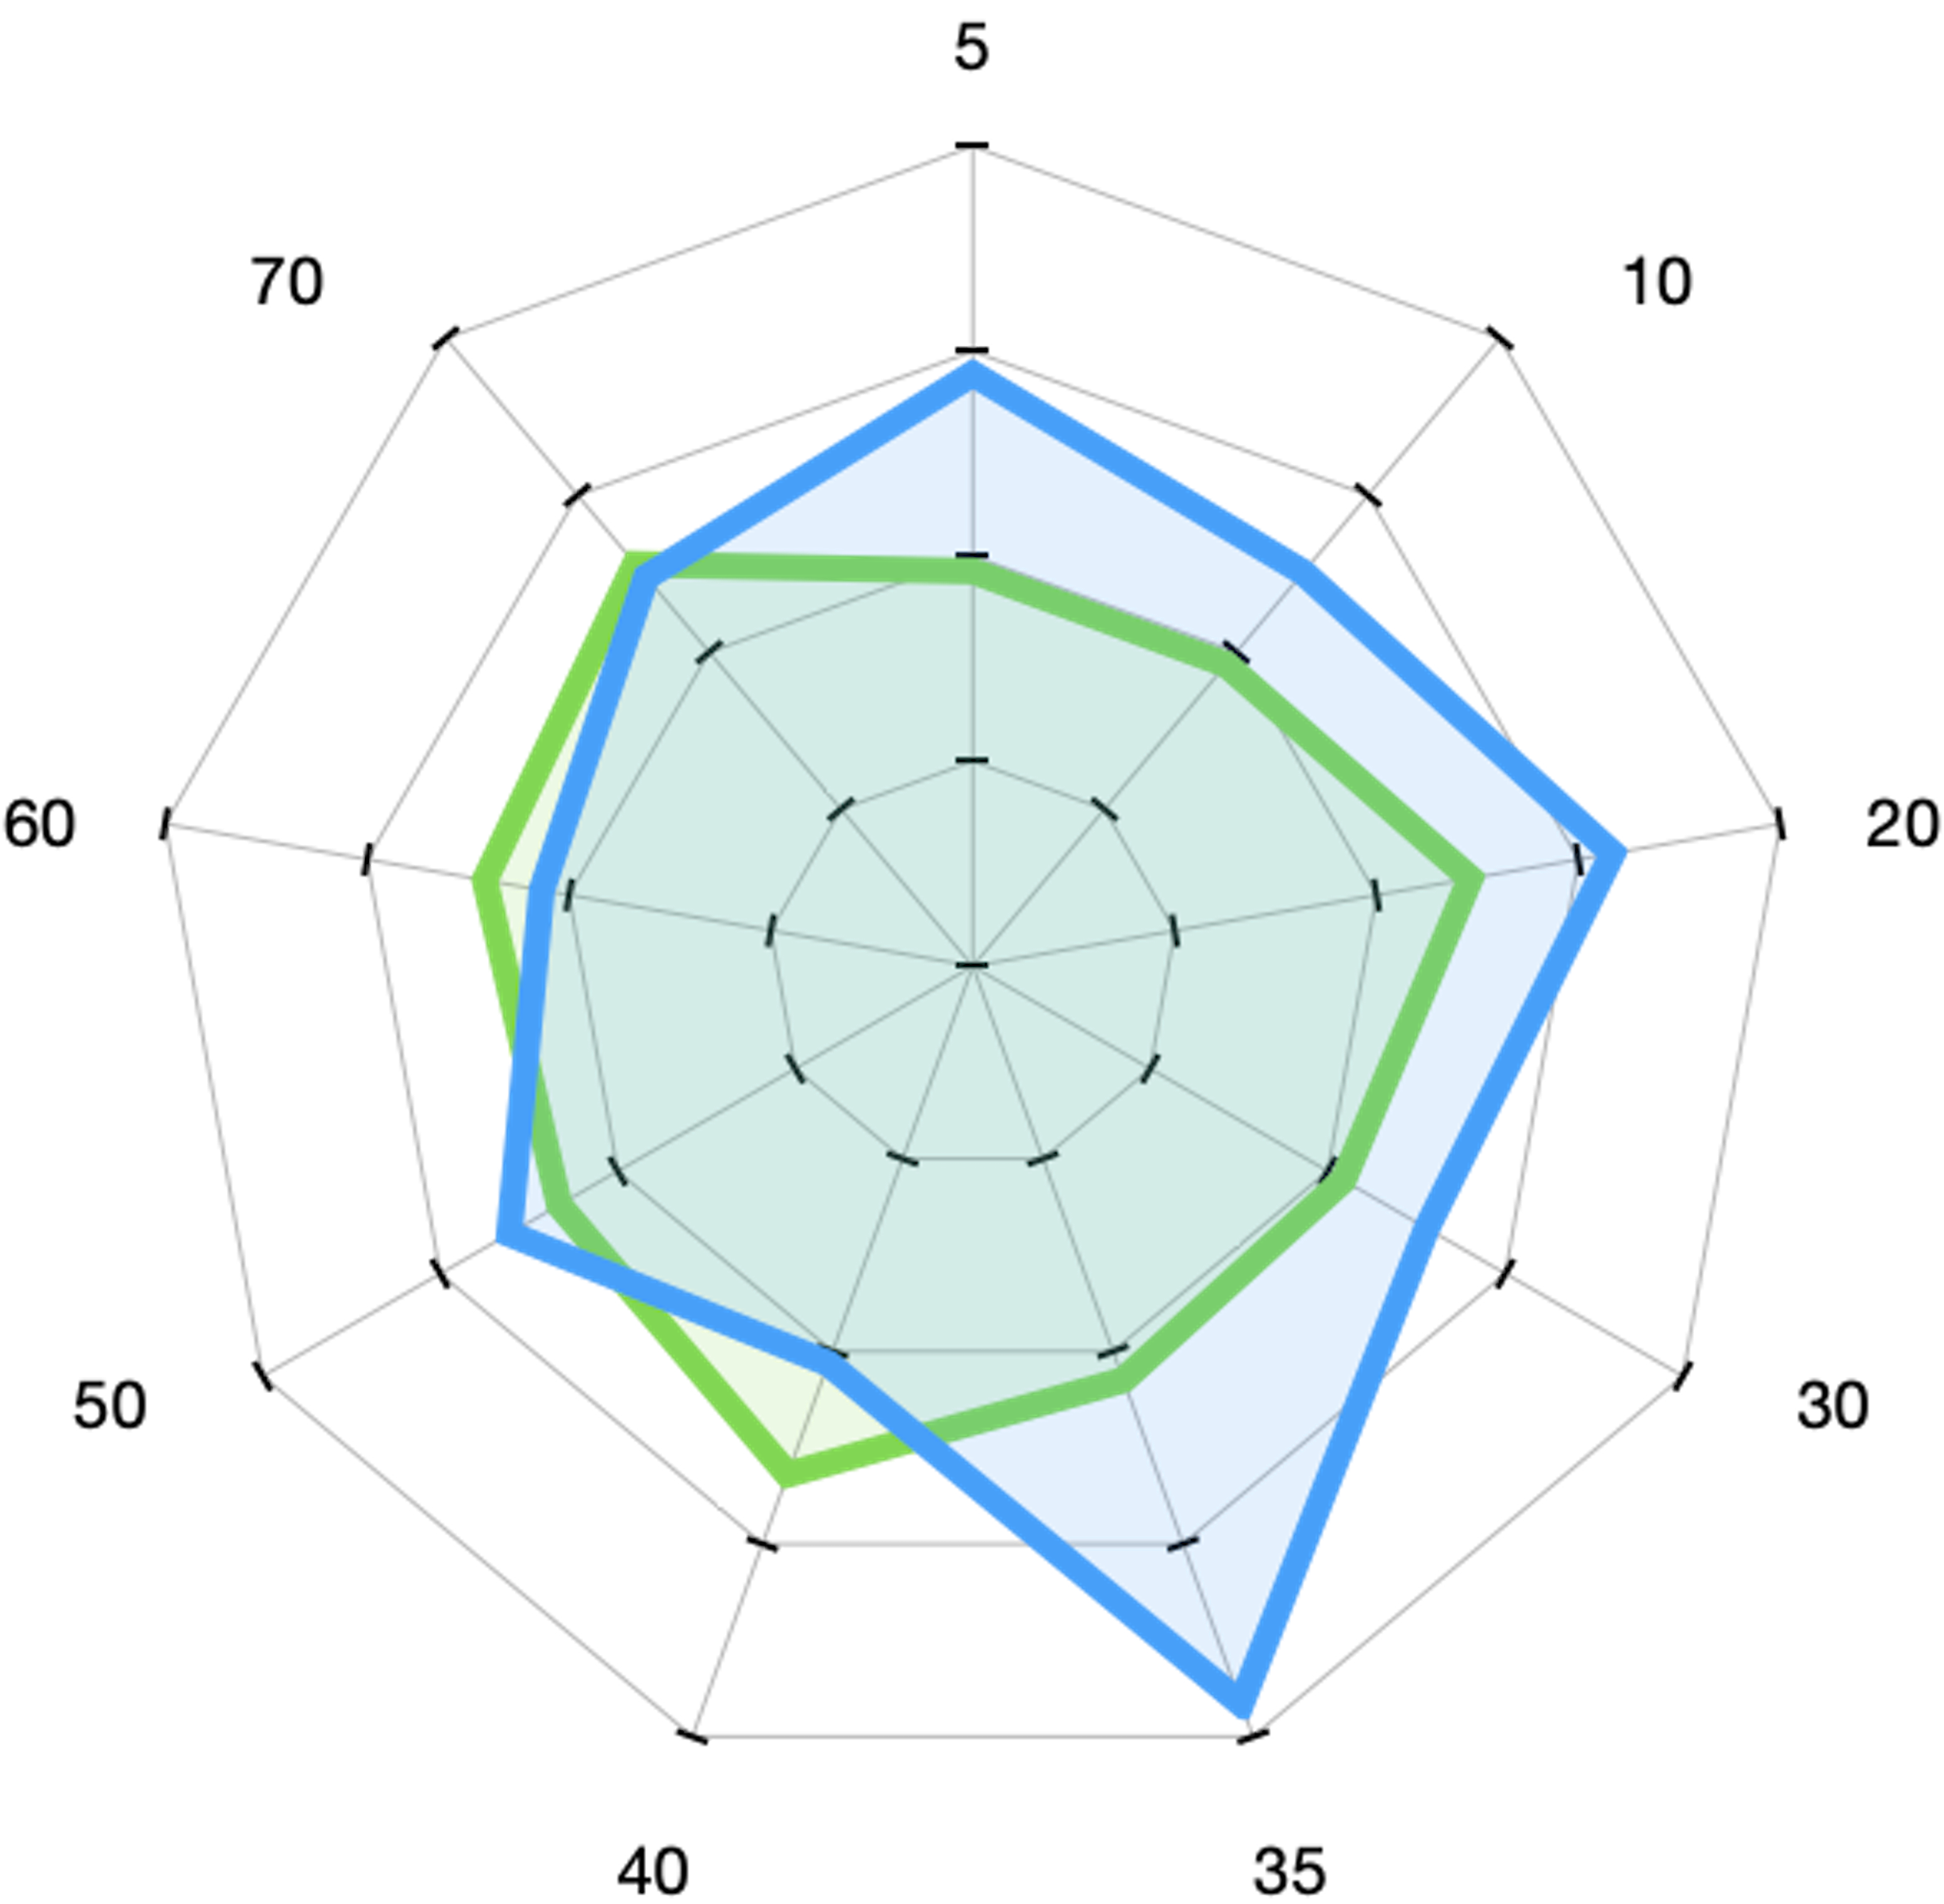
\includegraphics[width=0.4\textwidth, height=0.3\linewidth]{GRU_MAE_SPIDER.png}\label{fig:GRU_MAE_SPIDER}}
\caption{Performance comparison of Upward batch and Downward batch ensemble(UD-Batch) and Corresponding upward and downward ensemble(CUD-ensemble) using DL models over MAE performance measure.}
\label{fig:all_models_mae}
\end{figure}
%comparison of Upward batch and Downward batch ensemble(UD-Batch) and Corresponding upward and downward ensemble(CUD-ensemble) using DL models over MAE performance measure.

  

\begin{figure}[ht!]
%\centering
\subfloat[LSTM: UD-Batch ensemble Vs CUD ensemble]{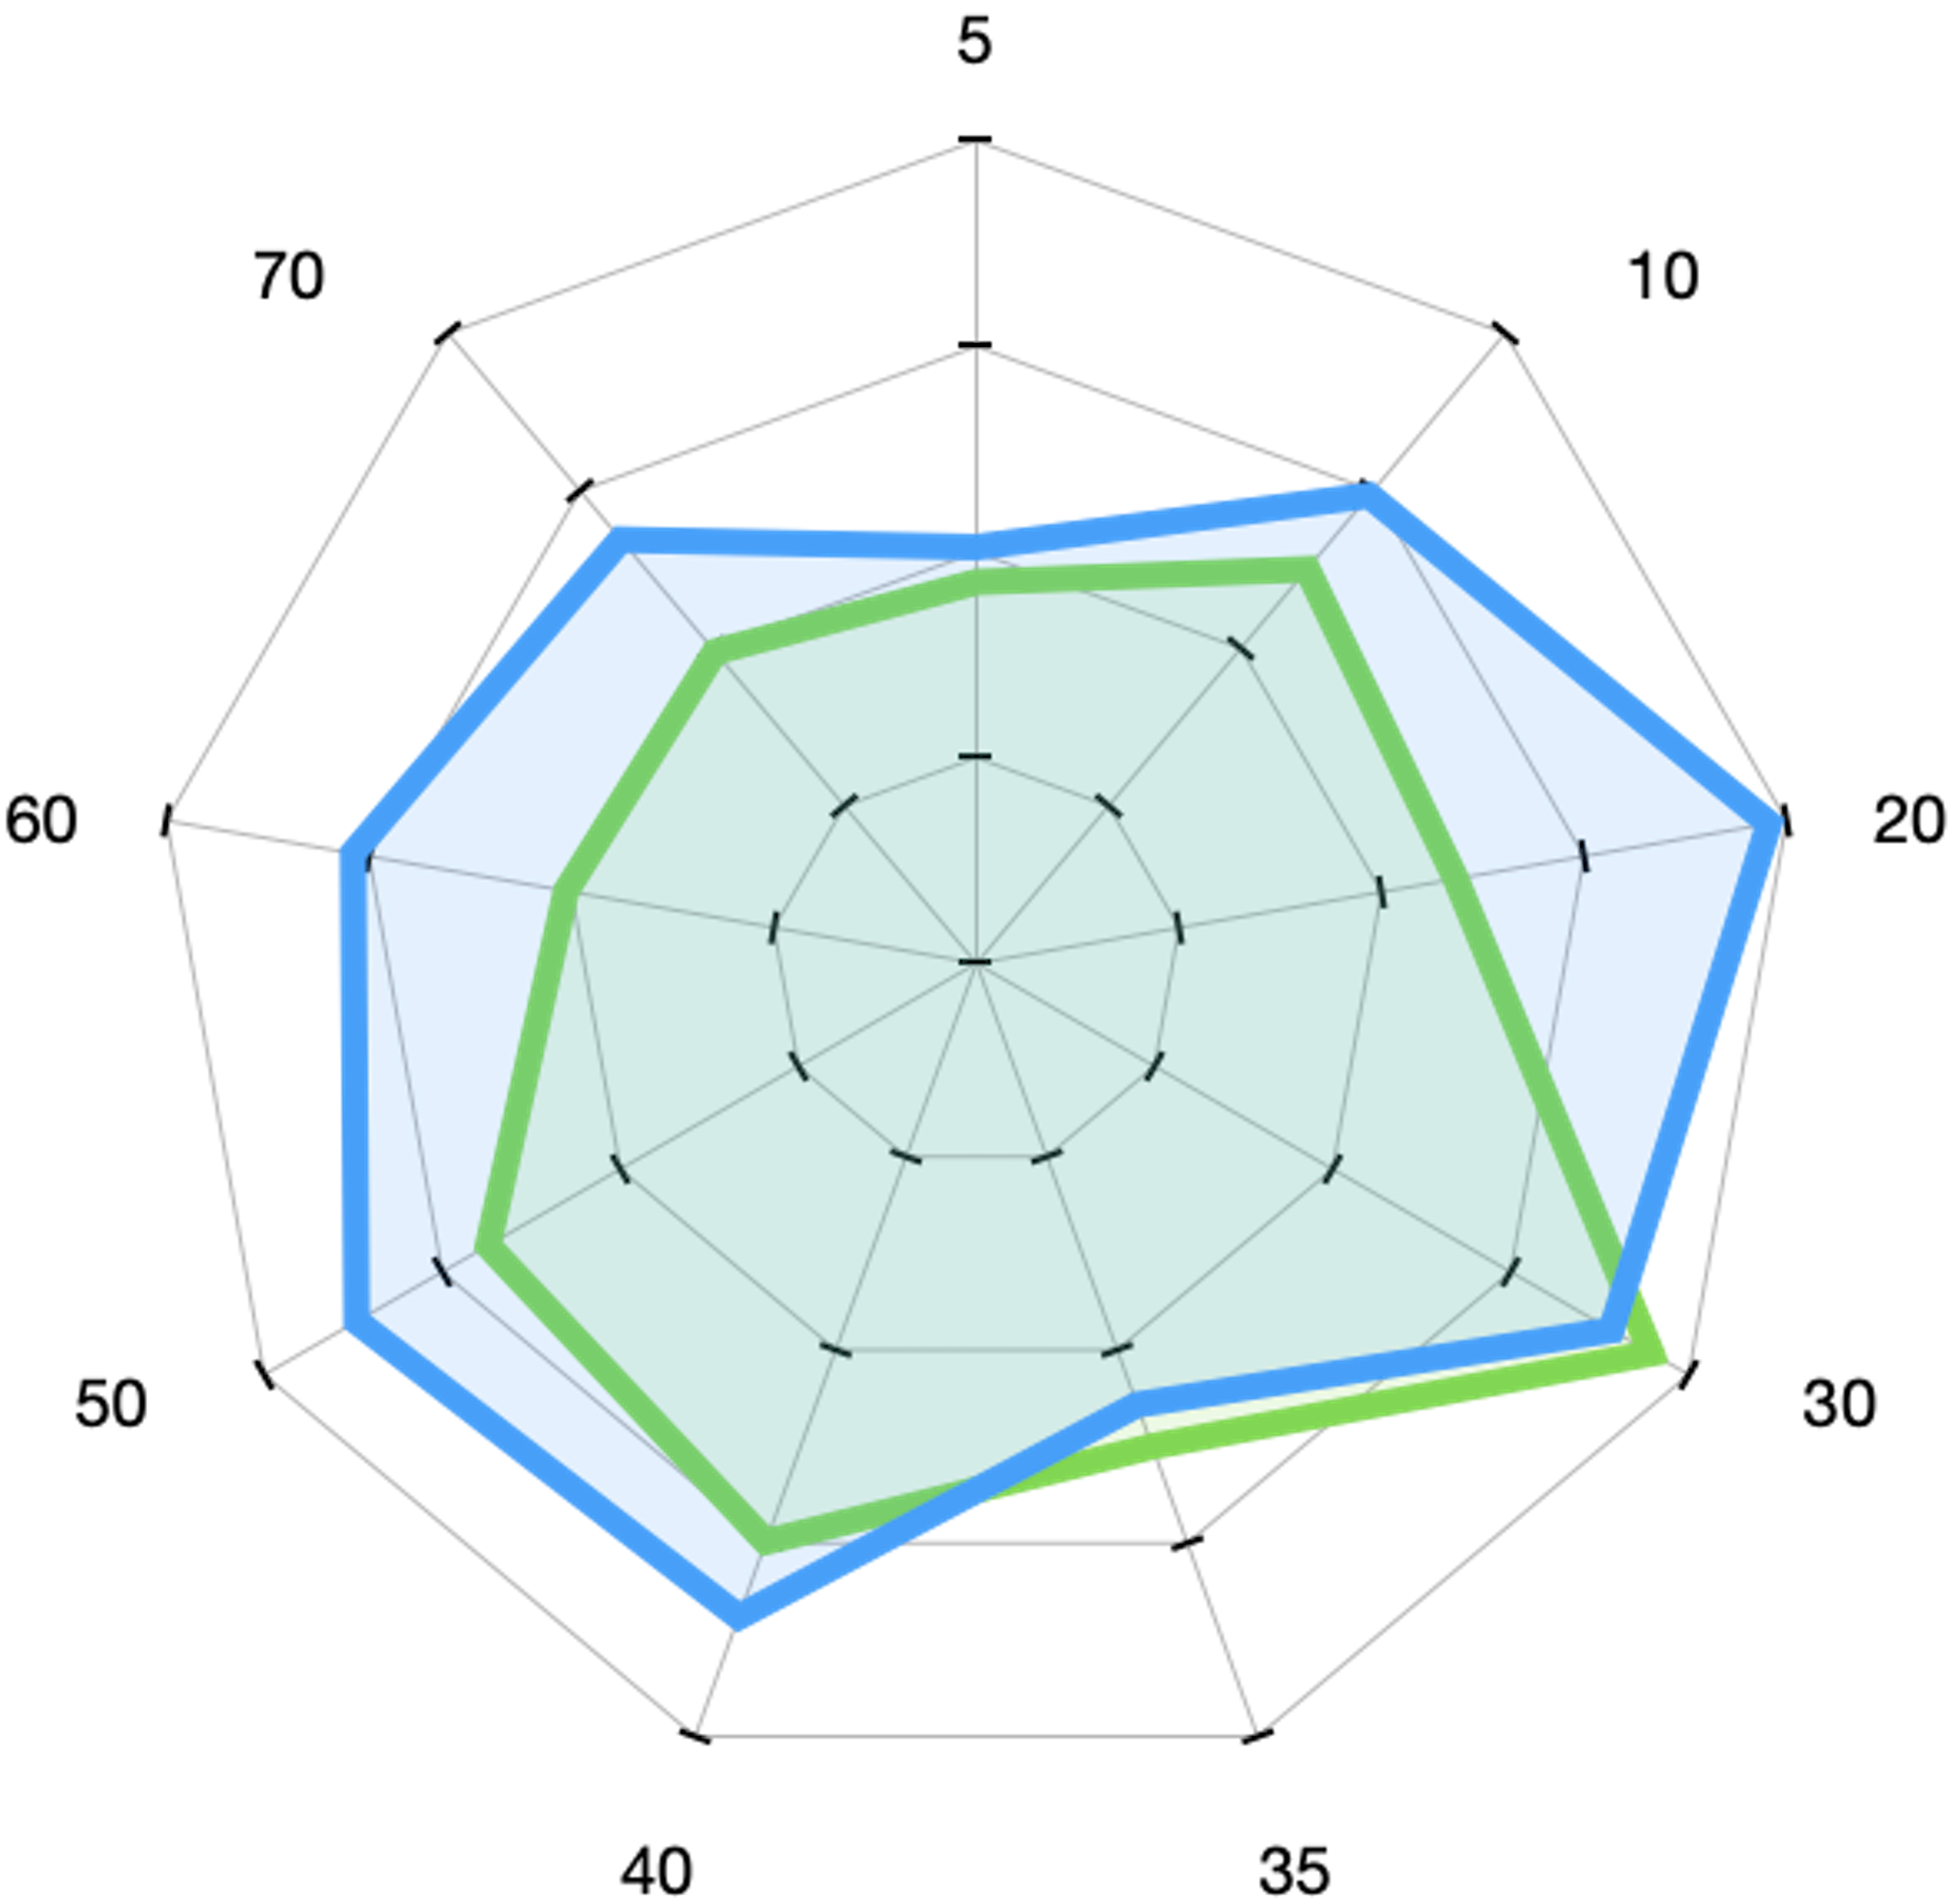
\includegraphics[scale=0.6]{LSTM_MSE_SPIDER.png}\label{fig:LSTM MSE SPIDER}}
\hfill
\subfloat[RNN: UD-Batch ensemble Vs CUD ensemble]{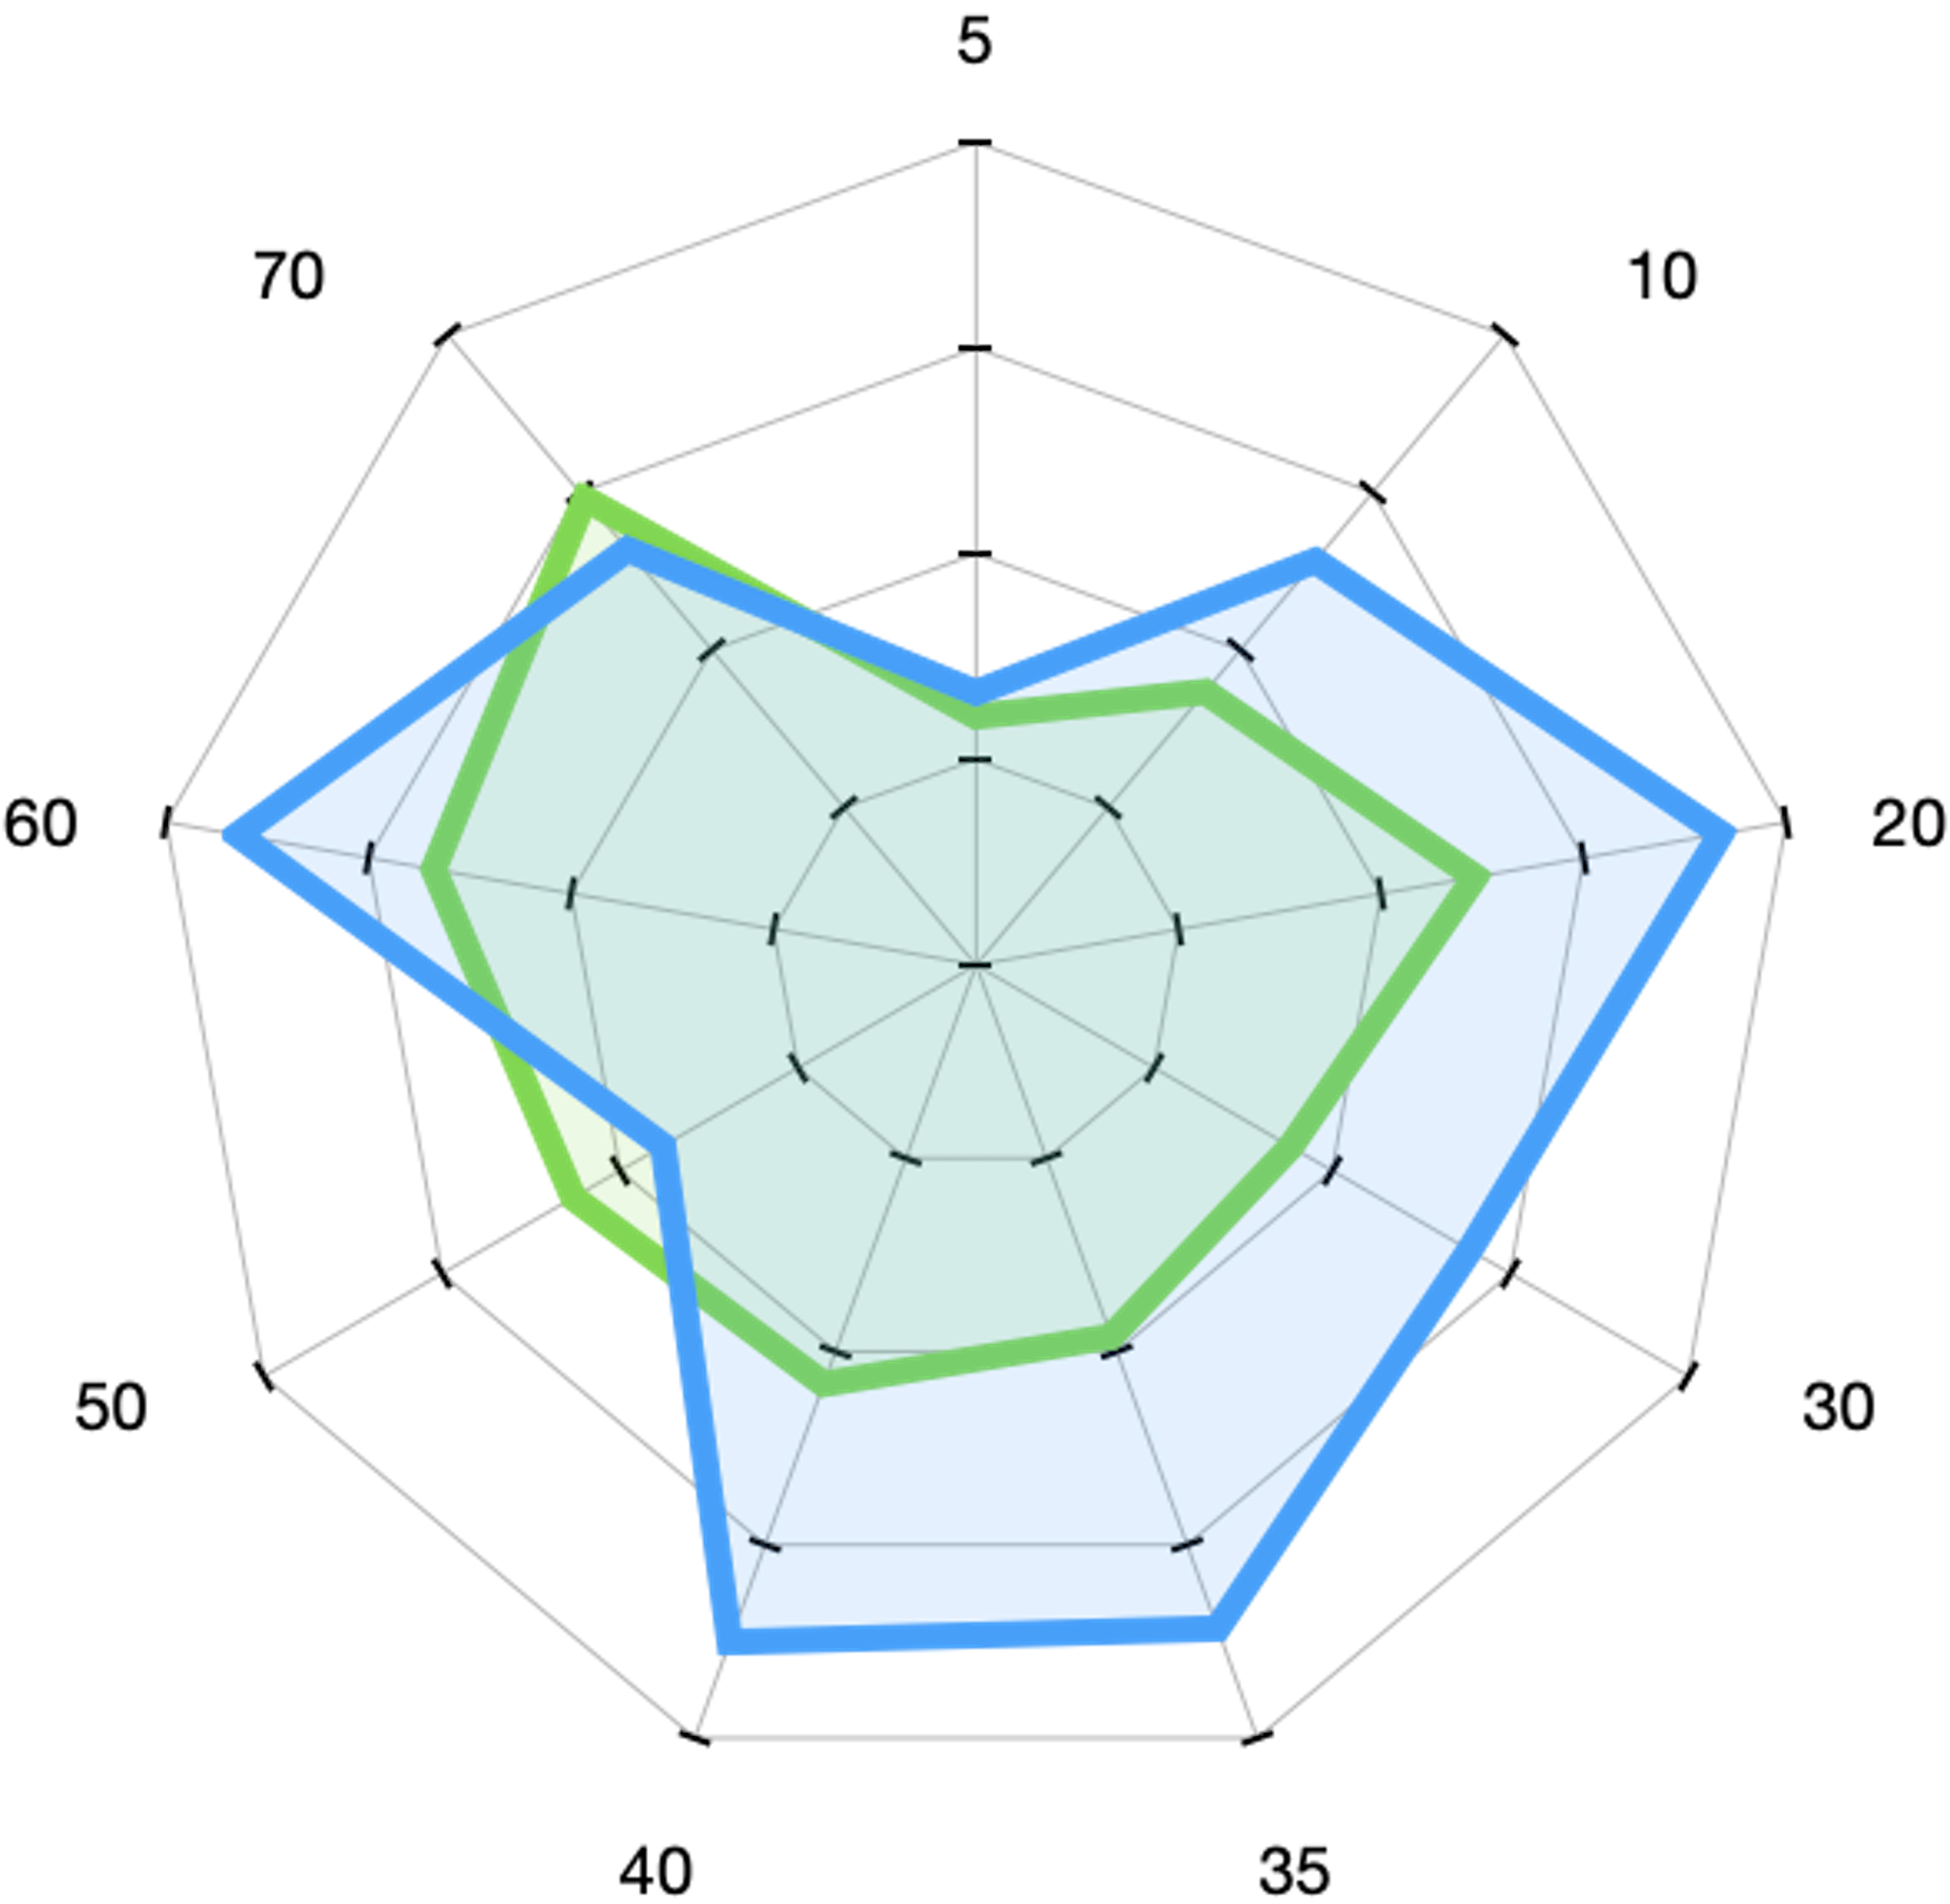
\includegraphics[scale=0.6]{RNN_MSE_SPIDER.png}\label{fig:RNN_MSE_SPIDER}}
% \vspace{\baselineskip} % Add vertical space between rows
\\
\subfloat[BiLSTM: UD-Batch ensemble Vs CUD ensemble]{\includegraphics[scale=0.6]{Bi-LSTM_MSE_SPIDER.png}\label{fig:BiLSTM_MSE_SPIDER}}
\hfill
\subfloat[GRU: UD-Batch ensemble Vs CUD ensemble]{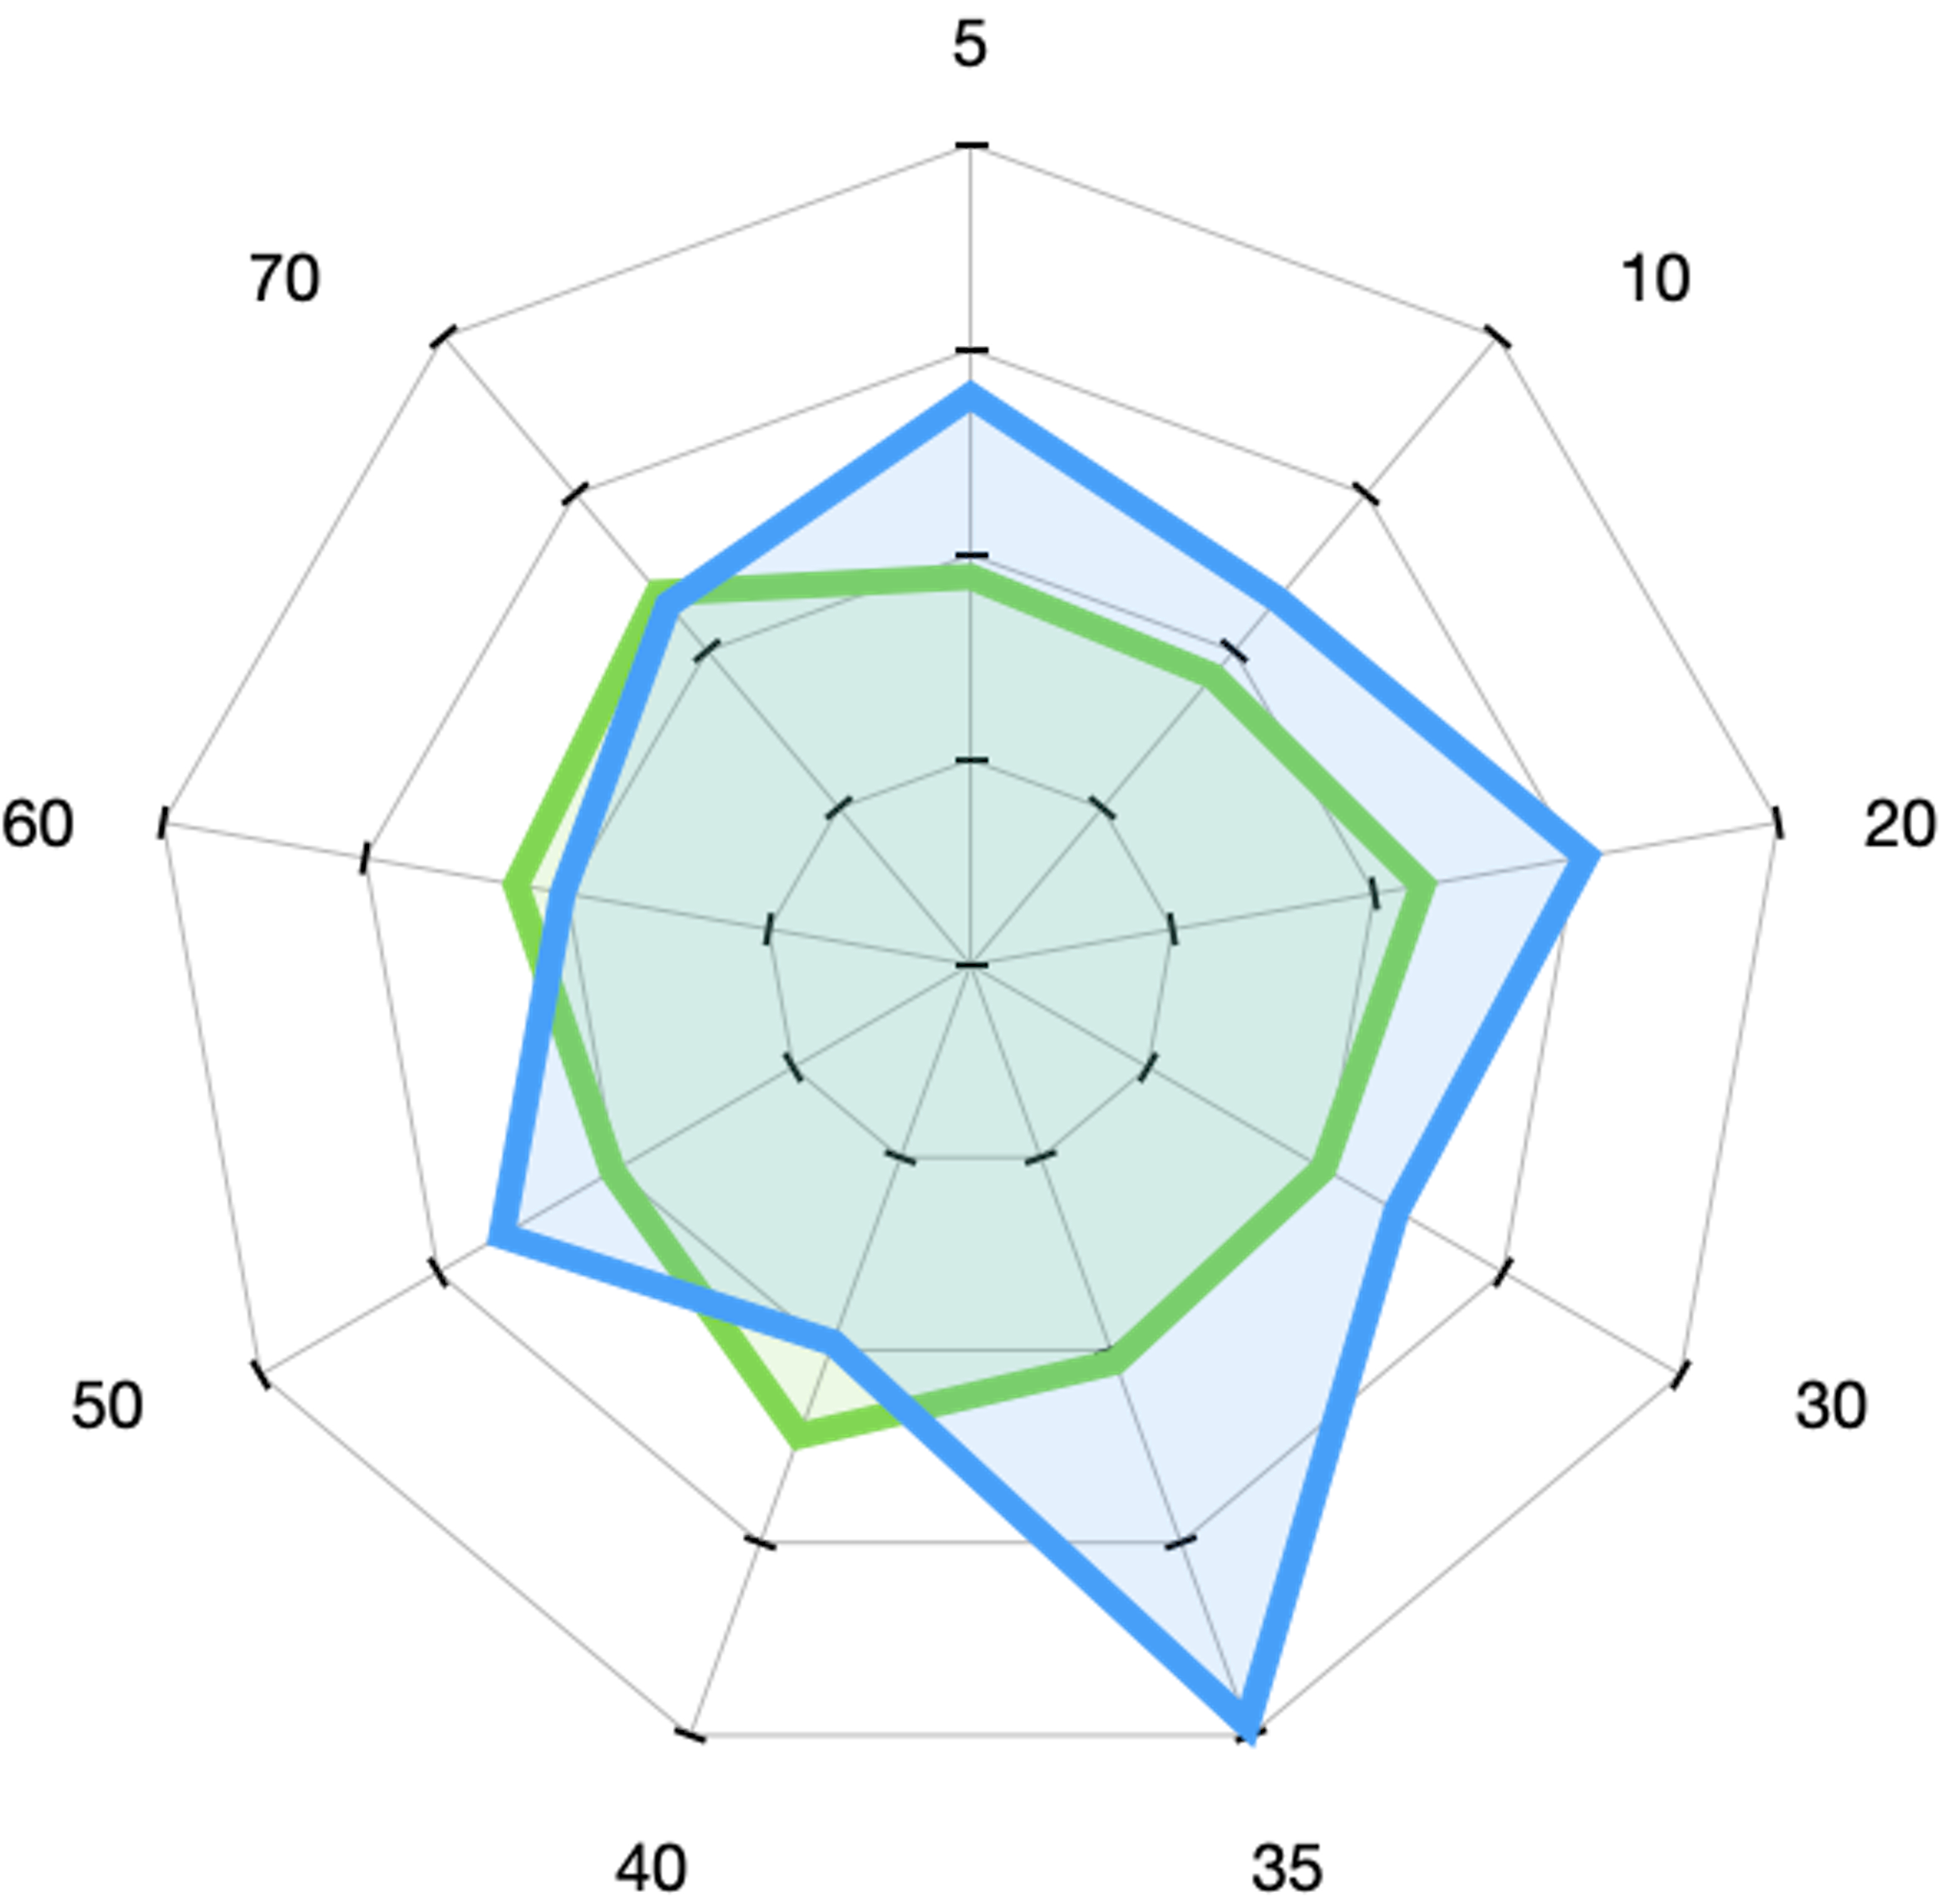
\includegraphics[scale=0.6]{GRU_MSE_SPIDER.png}\label{fig:GRU_MSE_SPIDER}}
\caption{Performance comparison of Upward batch and Downward batch ensemble(UD-Batch) and Corresponding upward and downward ensemble(CUD-ensemble) using DL models over MAE performance measure.}
\label{fig:all_models_mse}
\end{figure}


\begin{figure}[ht!]
%\centering
\subfloat[LSTM: UD-Batch ensemble Vs CUD ensemble]{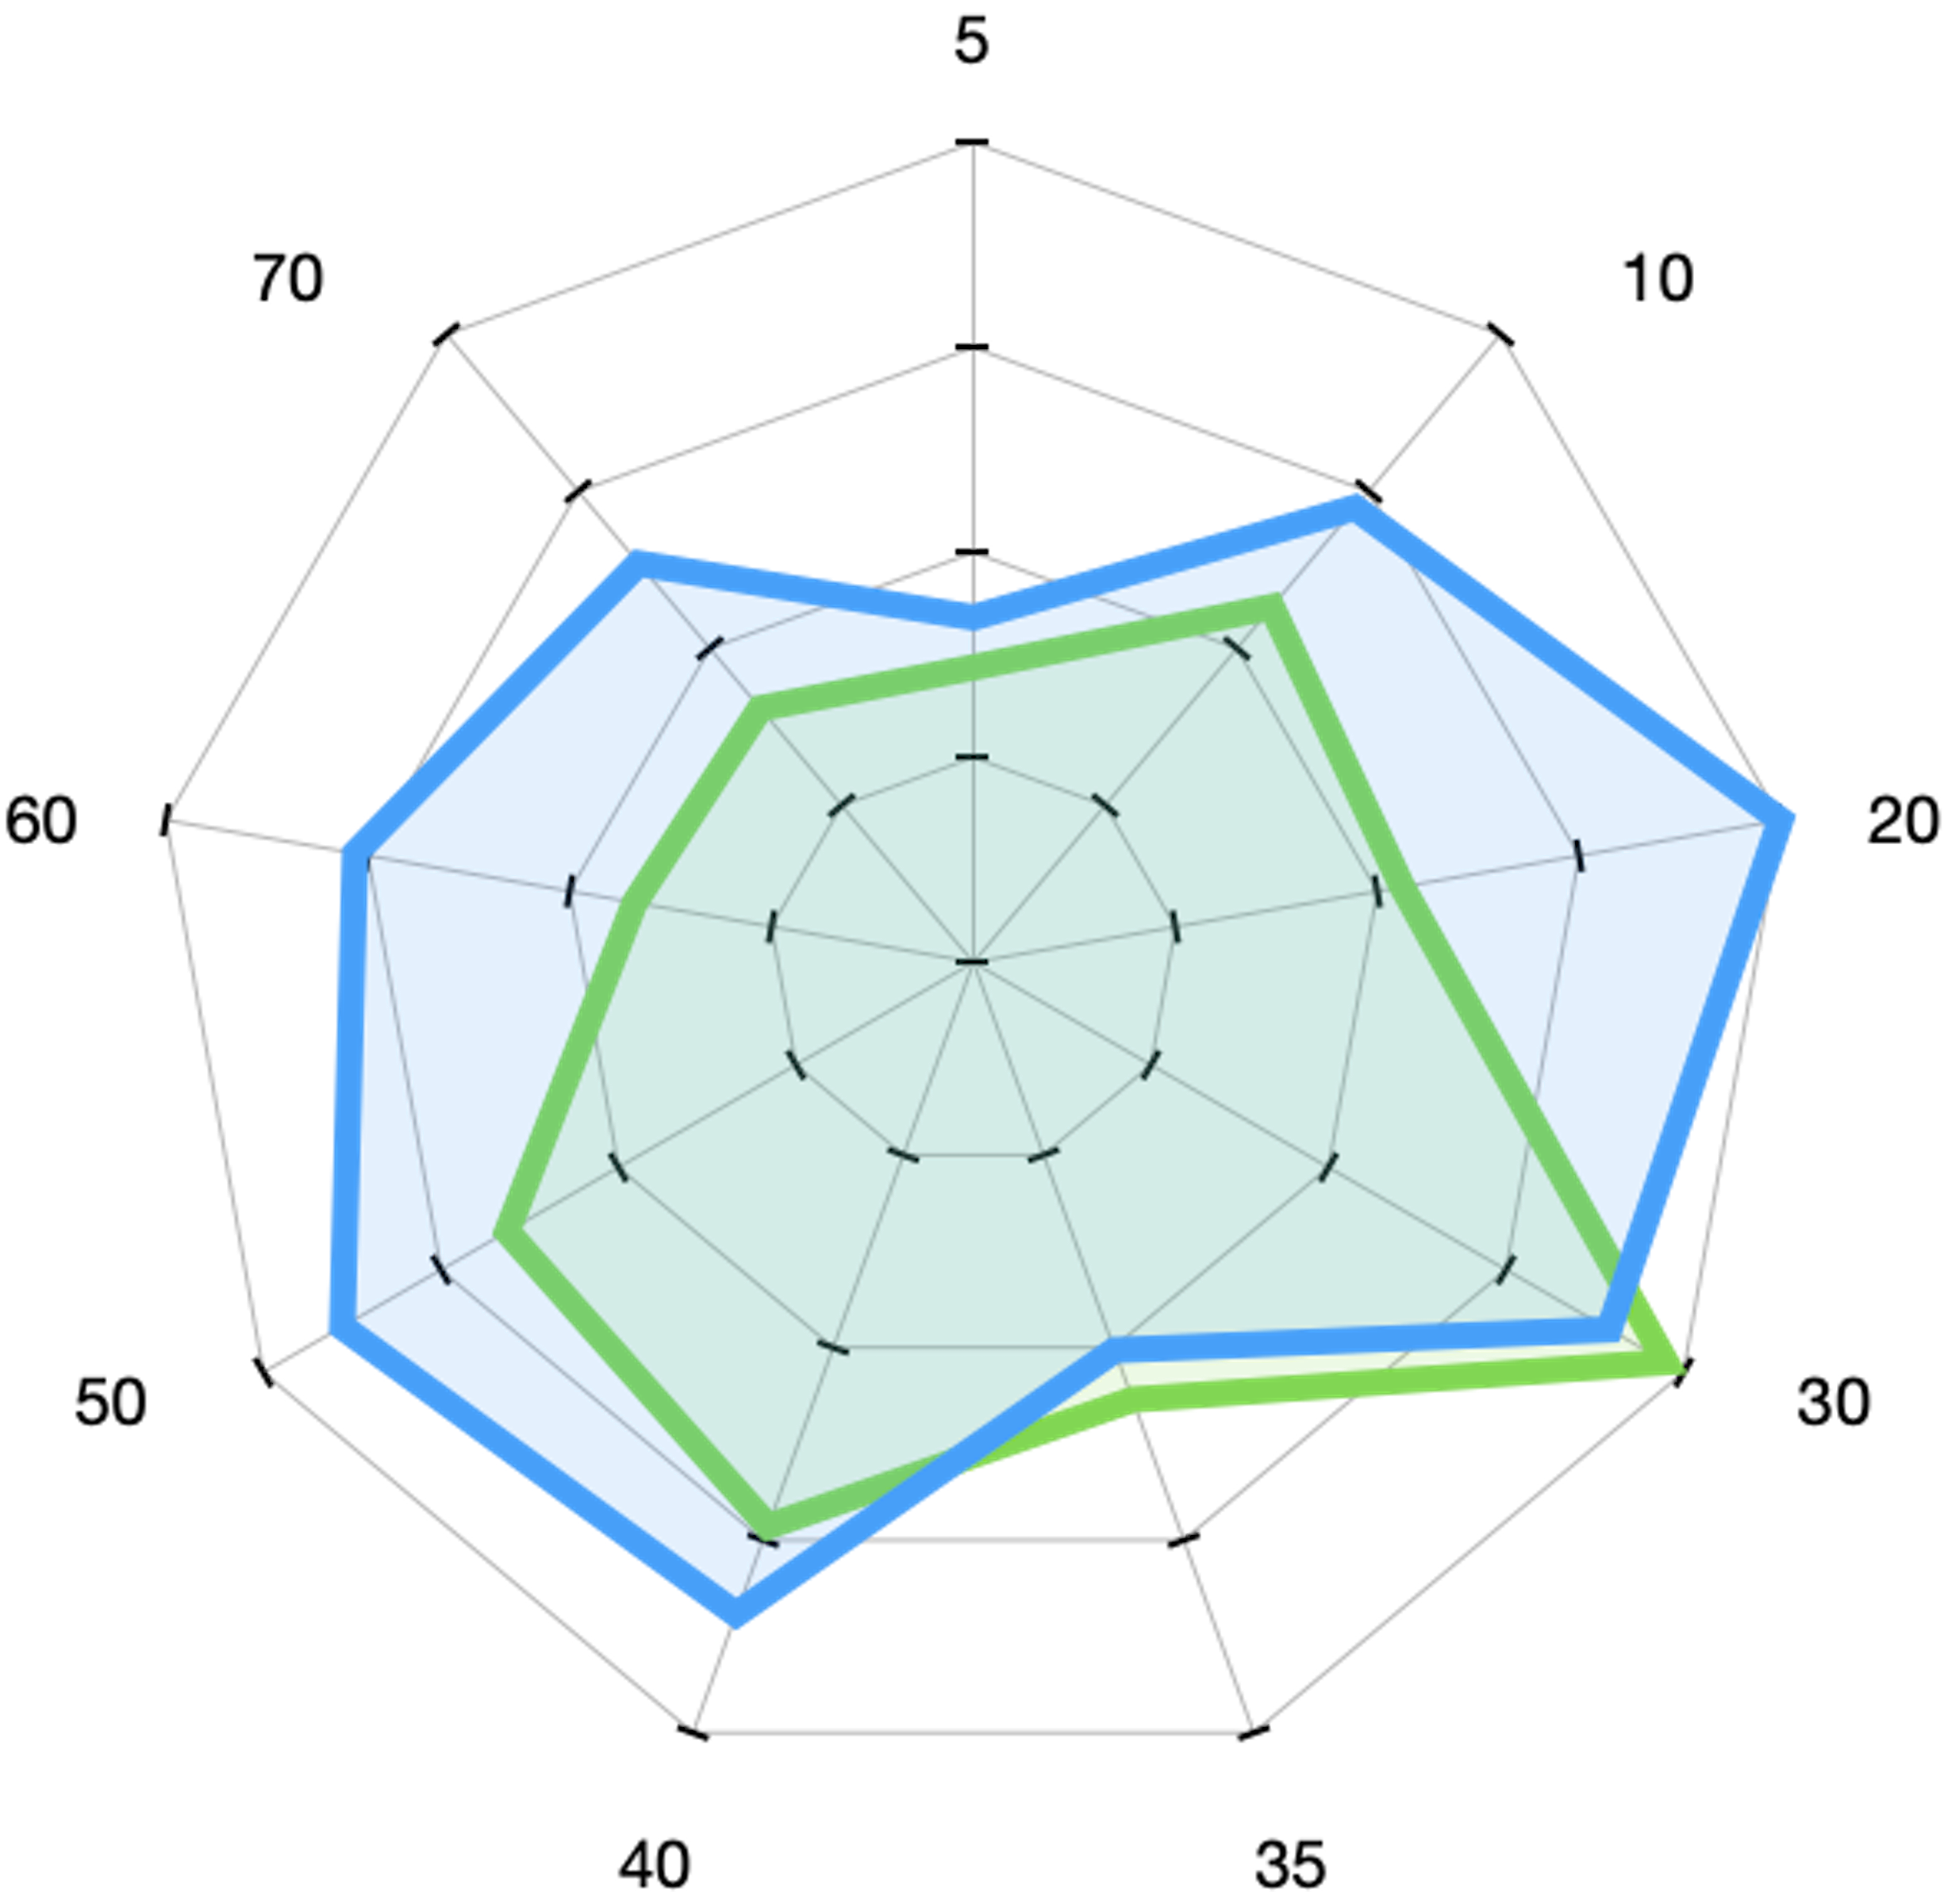
\includegraphics[scale=0.6]{LSTM_RMSE_SPIDER.png}\label{fig:LSTM RMSE SPIDER}}
\hfill
\subfloat[RNN: UD-Batch ensemble Vs CUD ensemble]{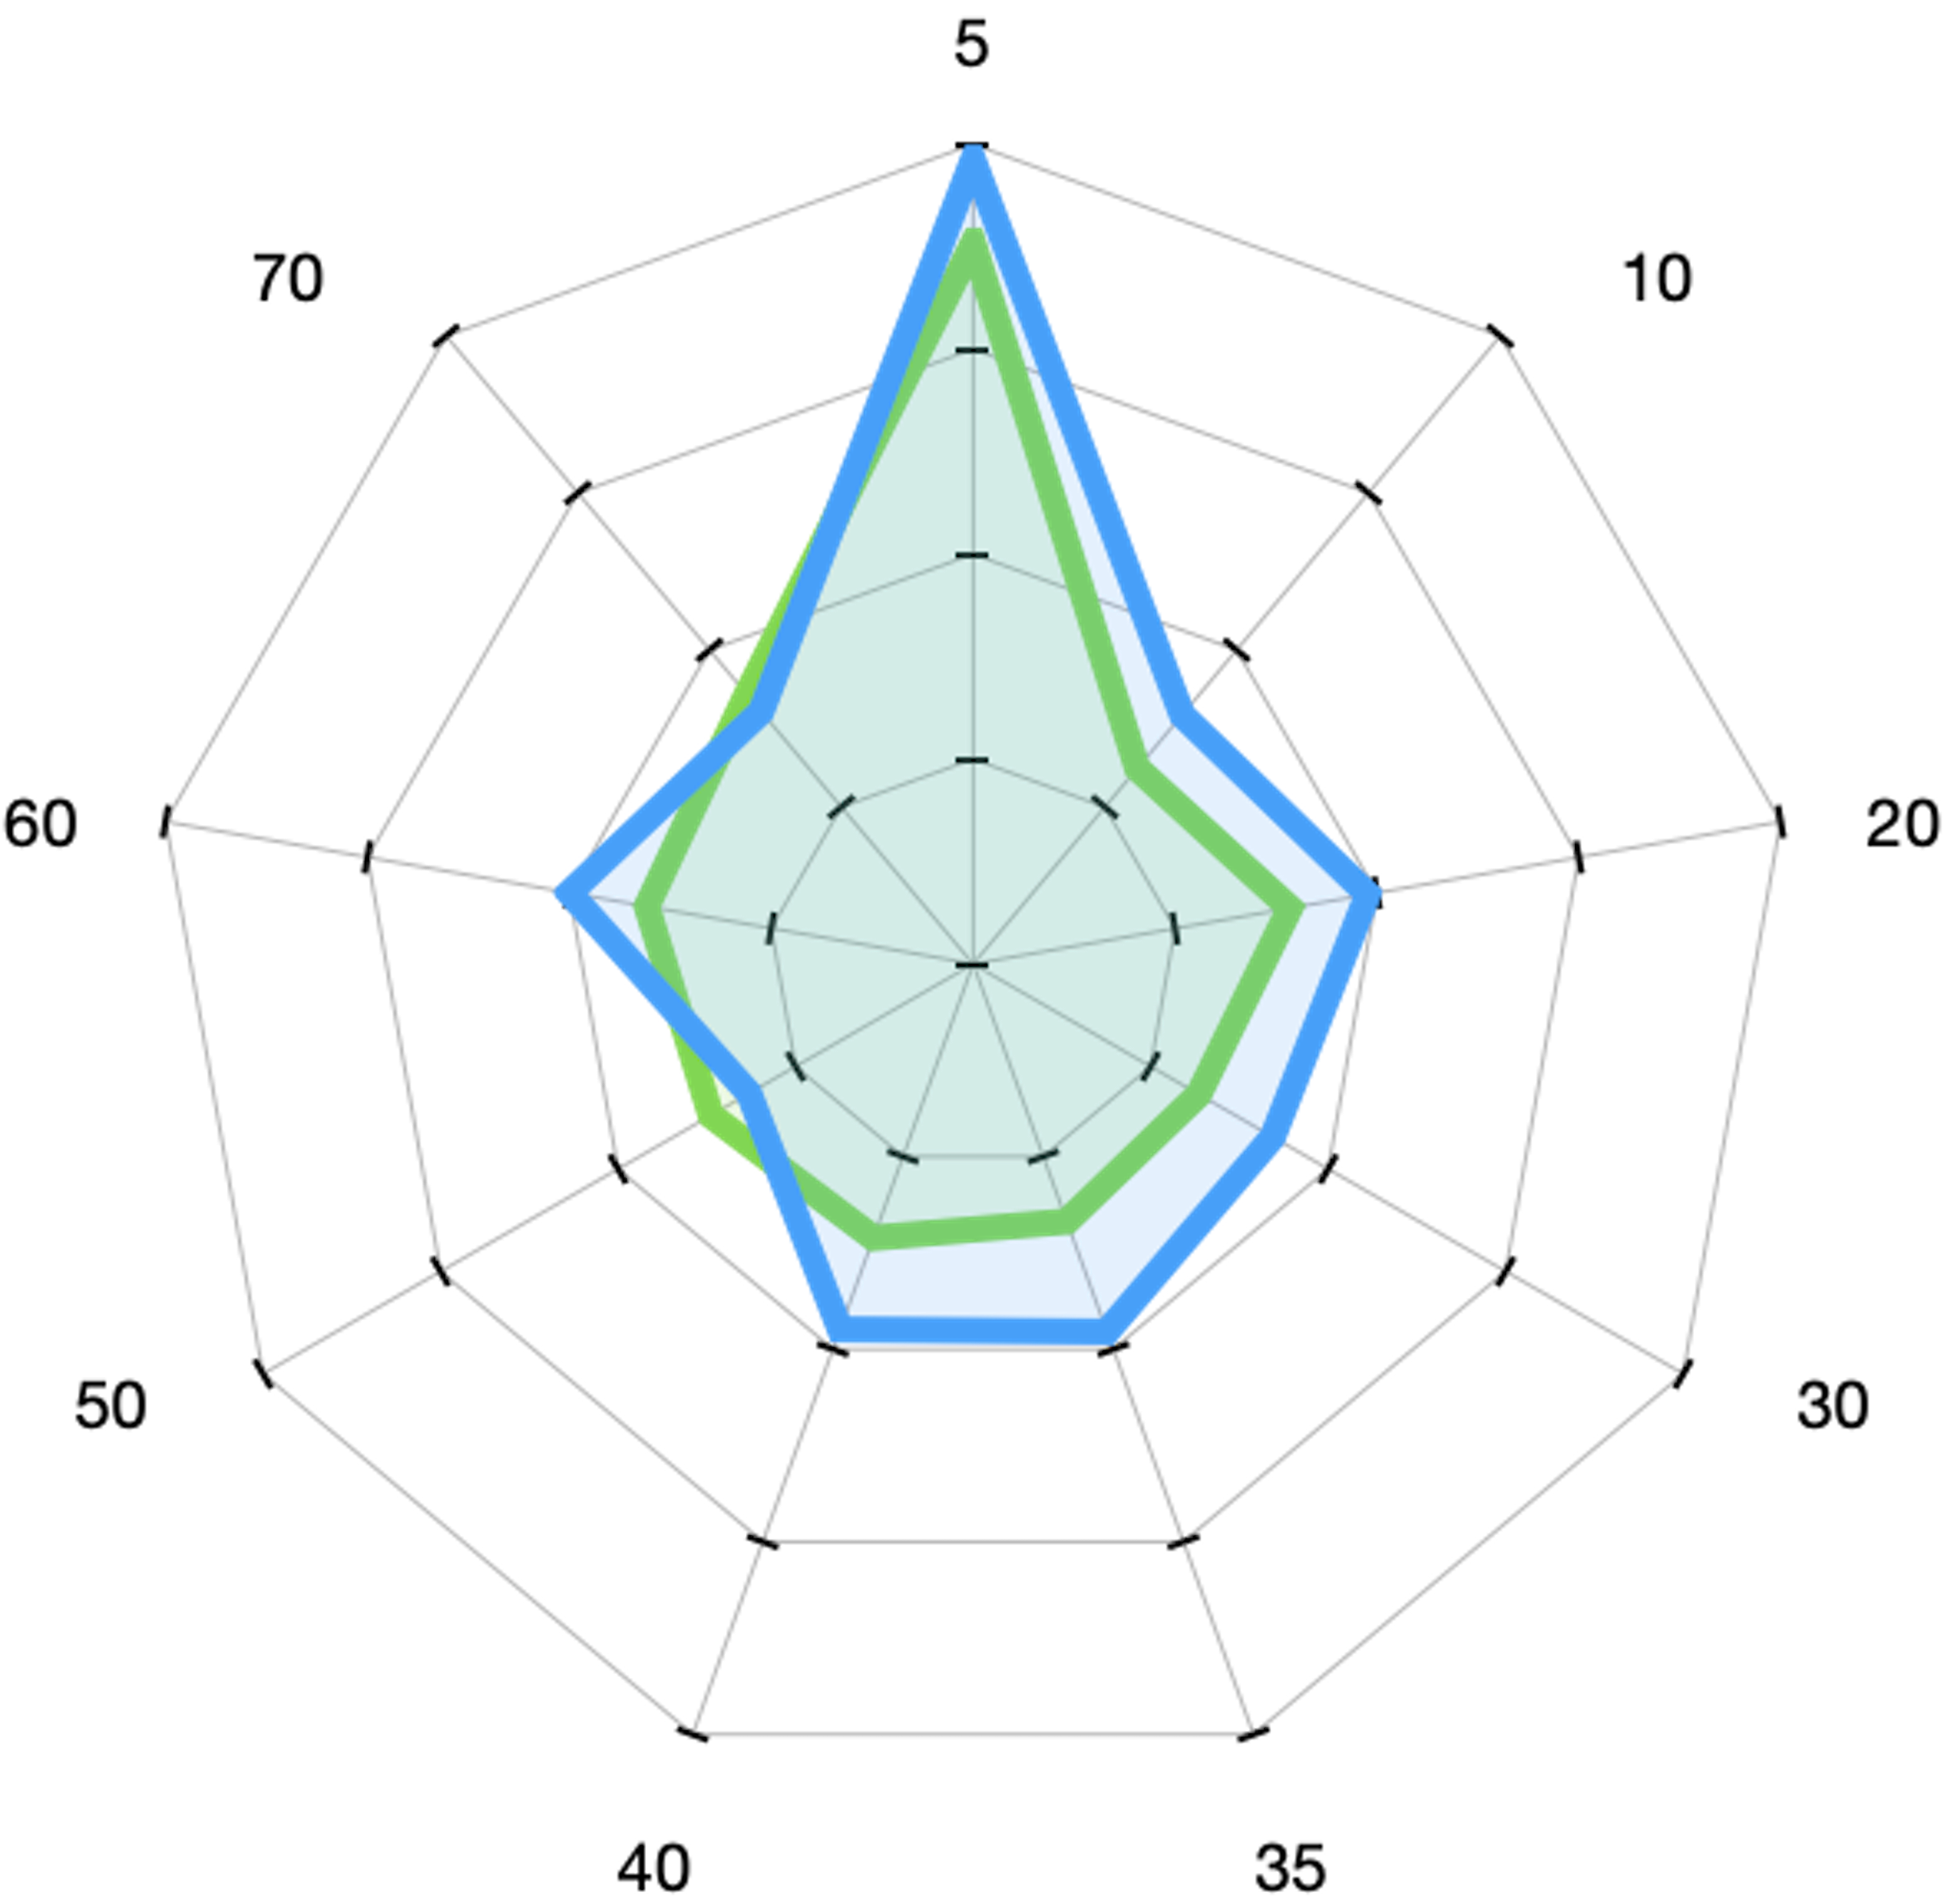
\includegraphics[scale=0.6]{RNN_RMSE_SPIDER.png}\label{fig:RNN_RMSE_SPIDER}}
\\
\subfloat[BiLSTM: UD-Batch ensemble Vs CUD ensemble]{\includegraphics[scale=0.6]{Bi-LSTM_RMSE_SPIDER.png}\label{fig:BiLSTM_RMSE_SPIDER}}
\hfill
\subfloat[GRU: UD-Batch ensemble Vs CUD ensemble]{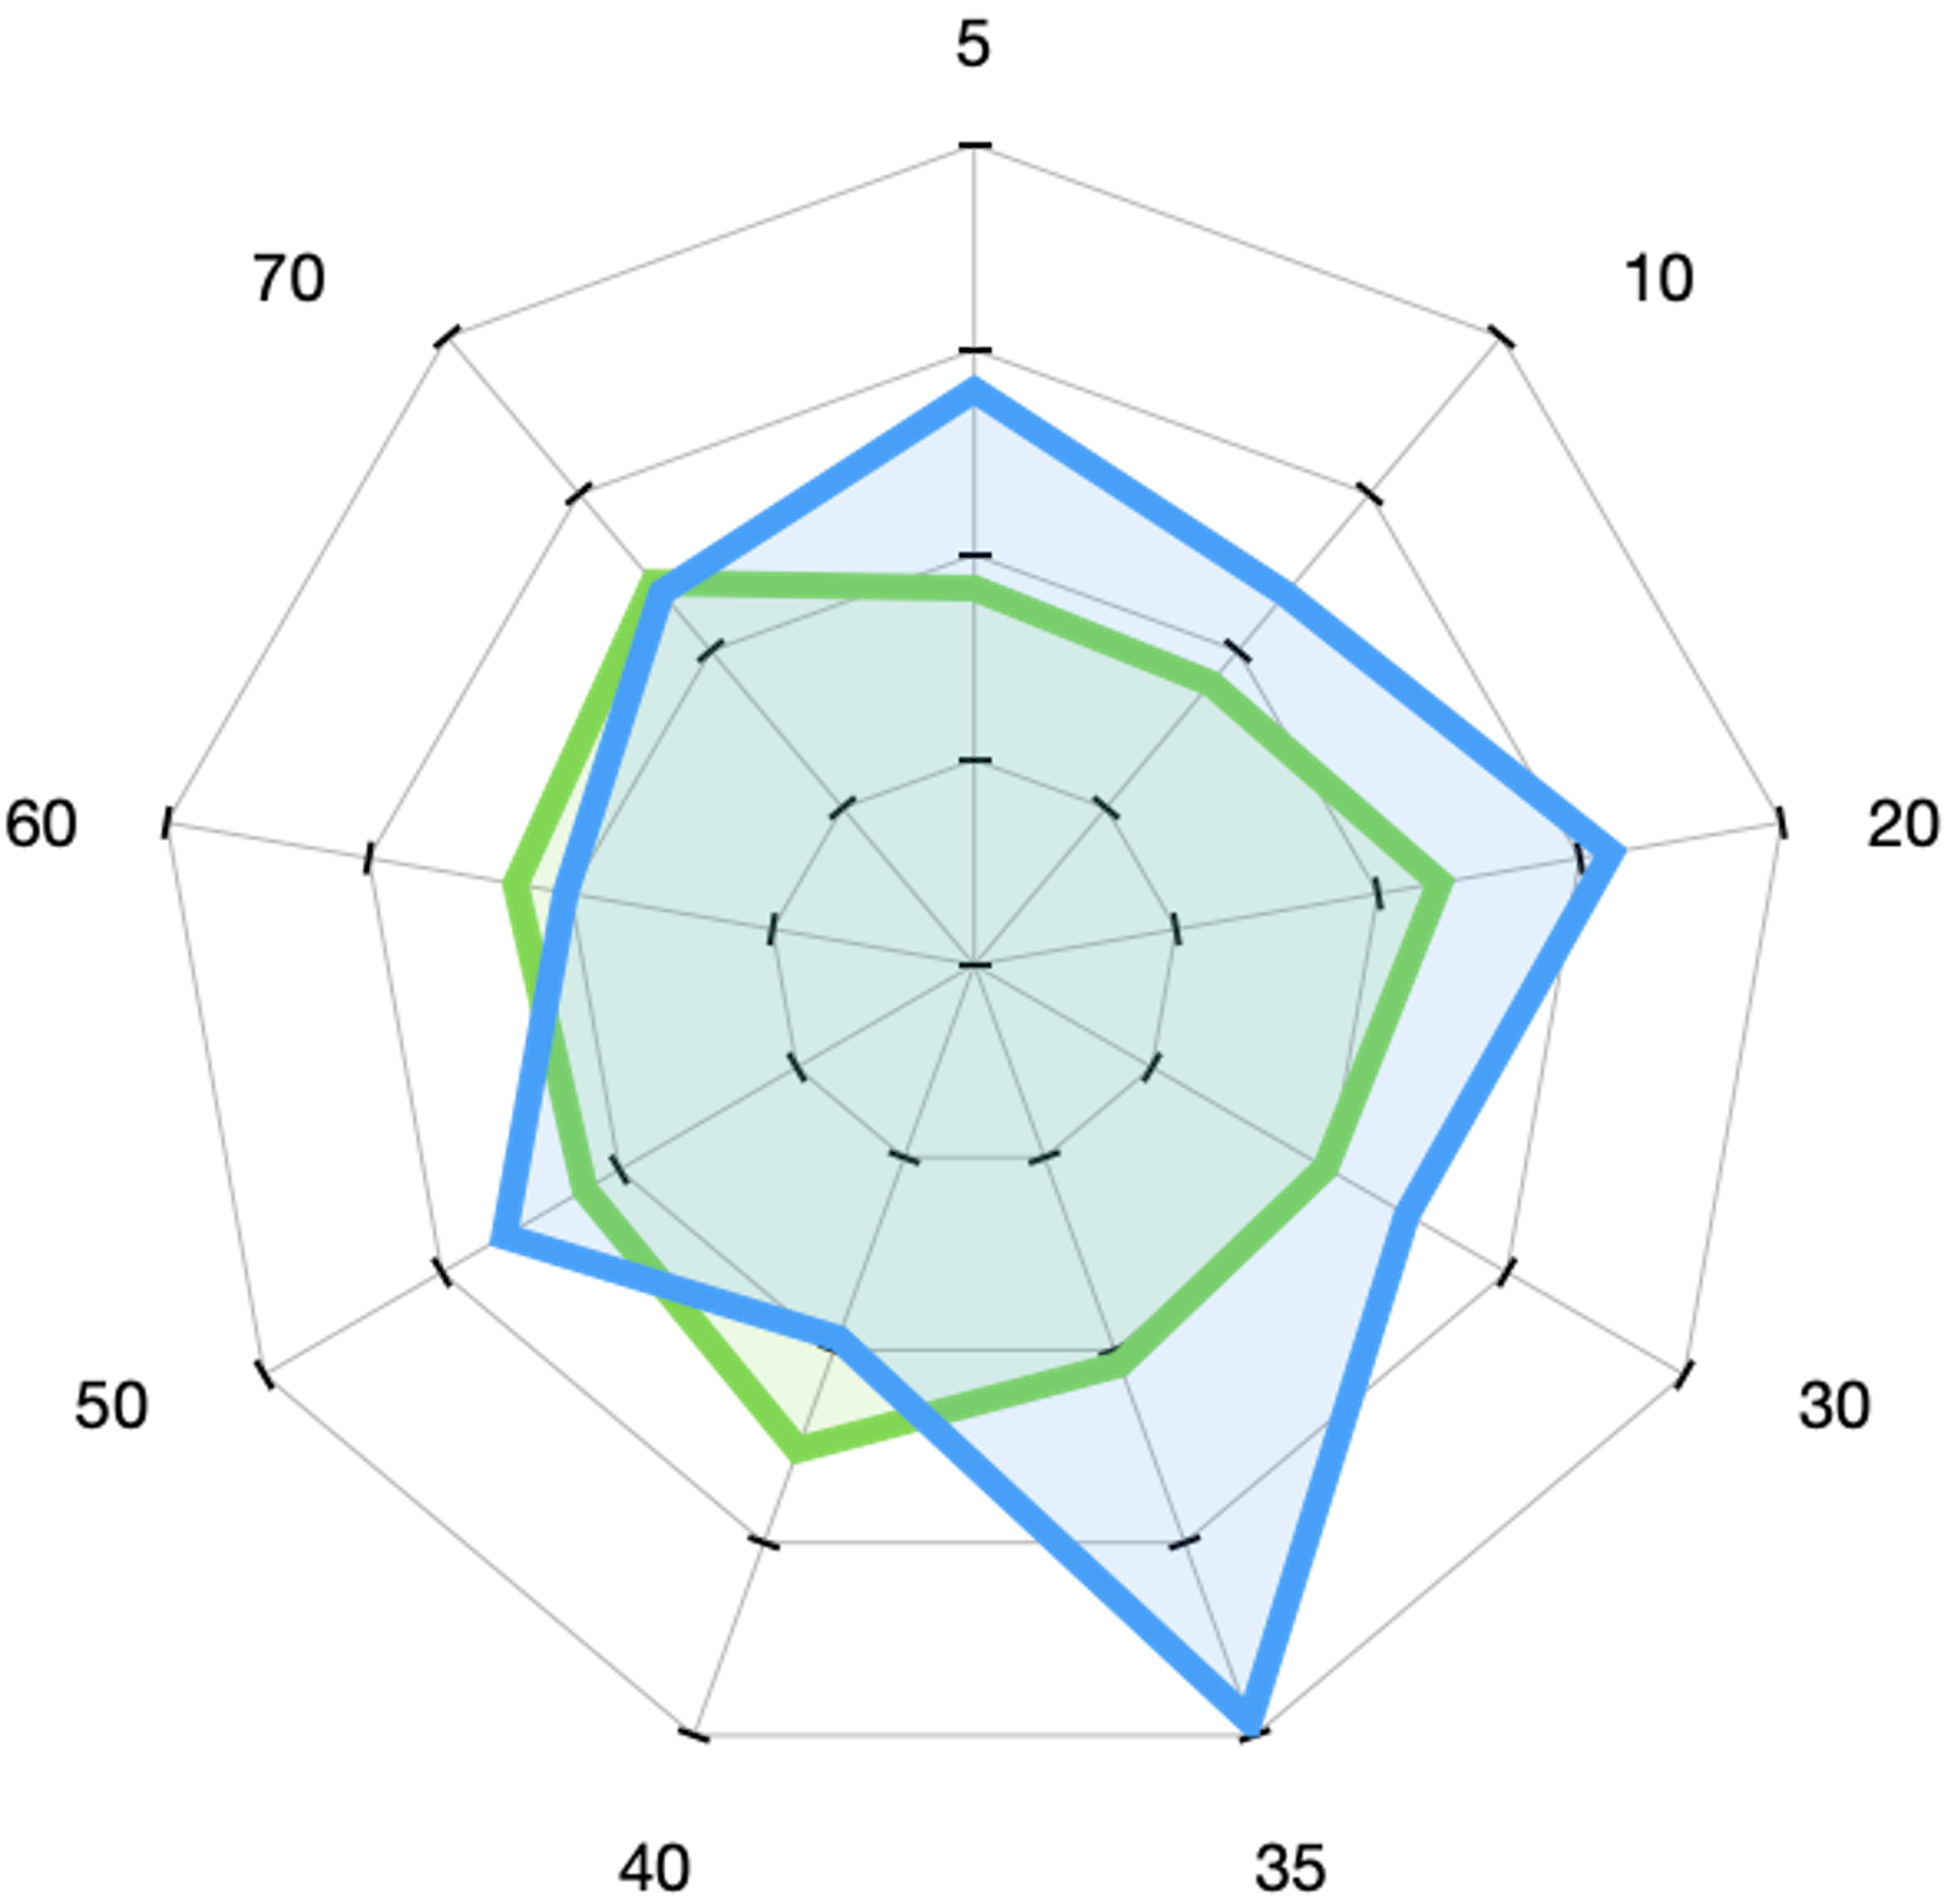
\includegraphics[scale=0.6]{GRU_RMSE_SPIDER.png}\label{fig:GRU_RMSE_SPIDER}}
\caption{Performance comparison of Upward batch and Downward batch ensemble(UD-Batch) and Corresponding upward and downward ensemble(CUD-ensemble) using DL models over RMSE performance measure.}
\label{fig:all_models_rmse}
\end{figure}


\begin{figure}[ht!]
%\centering
\subfloat[LSTM: UD-Batch ensemble Vs CUD ensemble]{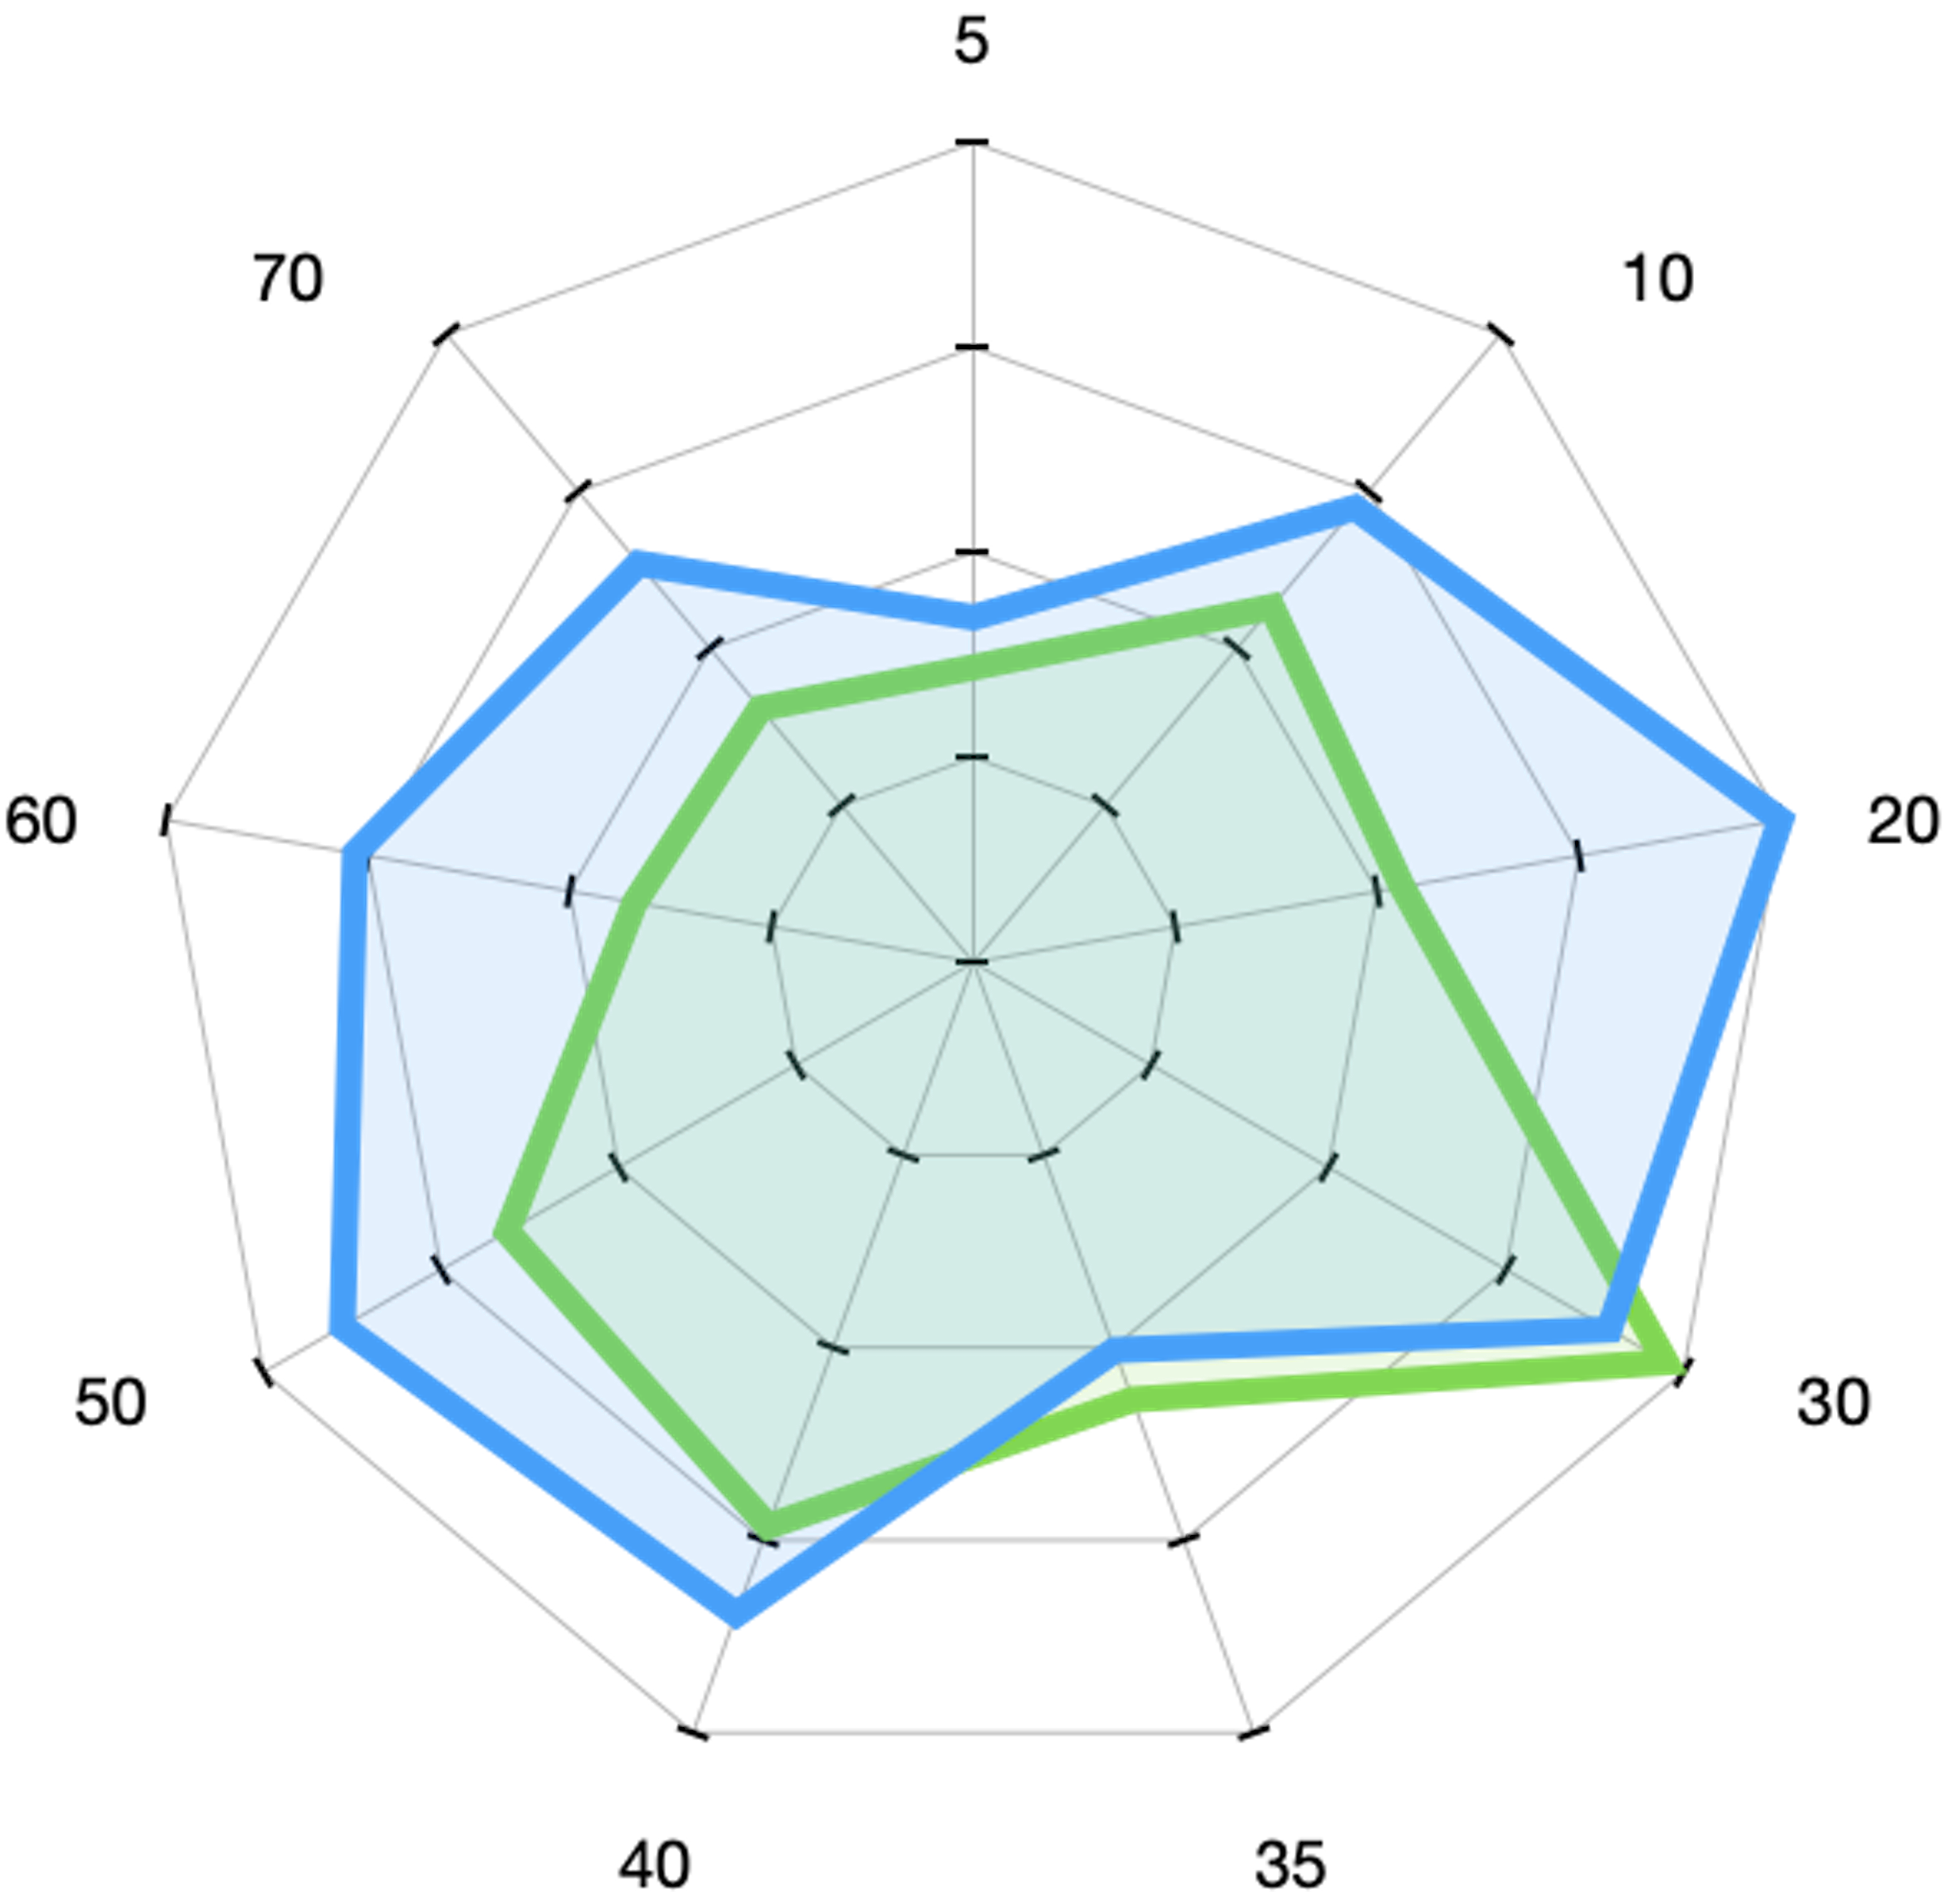
\includegraphics[scale=0.6]{LSTM_RMSE_SPIDER.png}\label{fig:LSTM MAPE SPIDER}}
\hfill
\subfloat[RNN: UD-Batch ensemble Vs CUD ensemble]{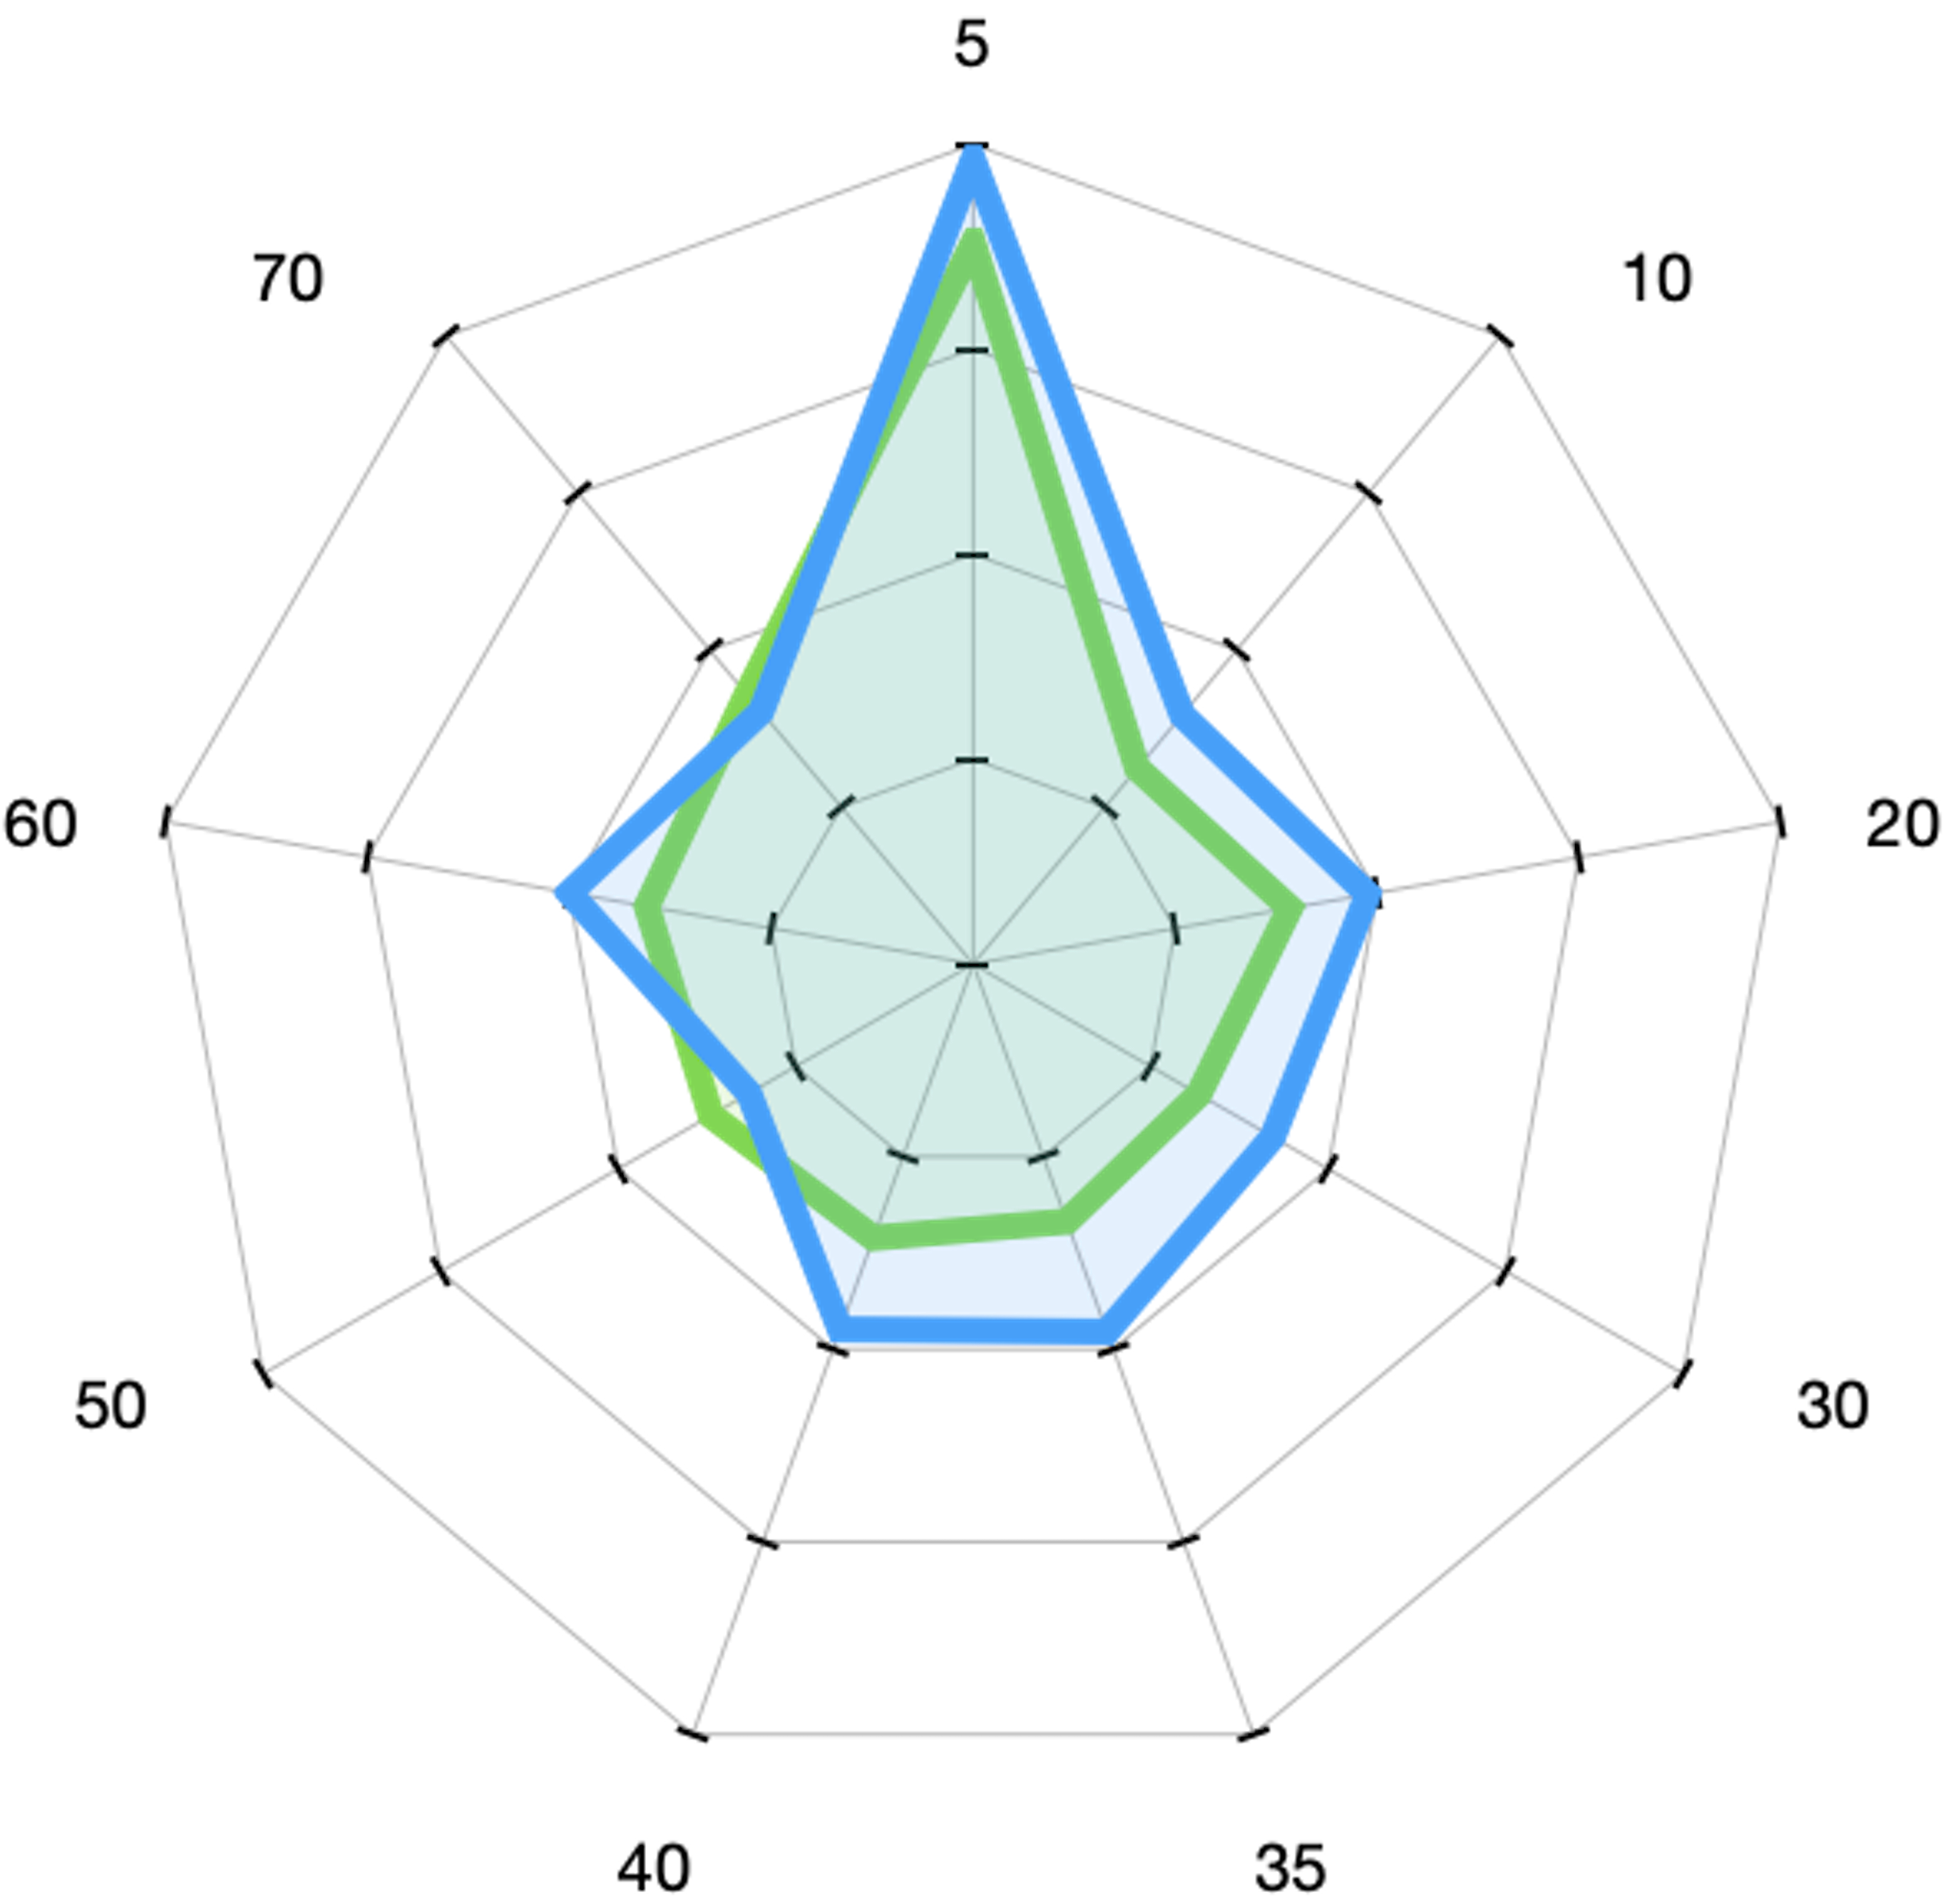
\includegraphics[scale=0.6]{RNN_RMSE_SPIDER.png}\label{fig:RNN_MAPE_SPIDER}}
\\
\subfloat[BiLSTM: UD-Batch ensemble Vs CUD ensemble]{\includegraphics[scale=0.6]{Bi-LSTM_RMSE_SPIDER.png}\label{fig:BiLSTM_MAPE_SPIDER}}
\hfill
\subfloat[GRU: UD-Batch ensemble Vs CUD ensemble]{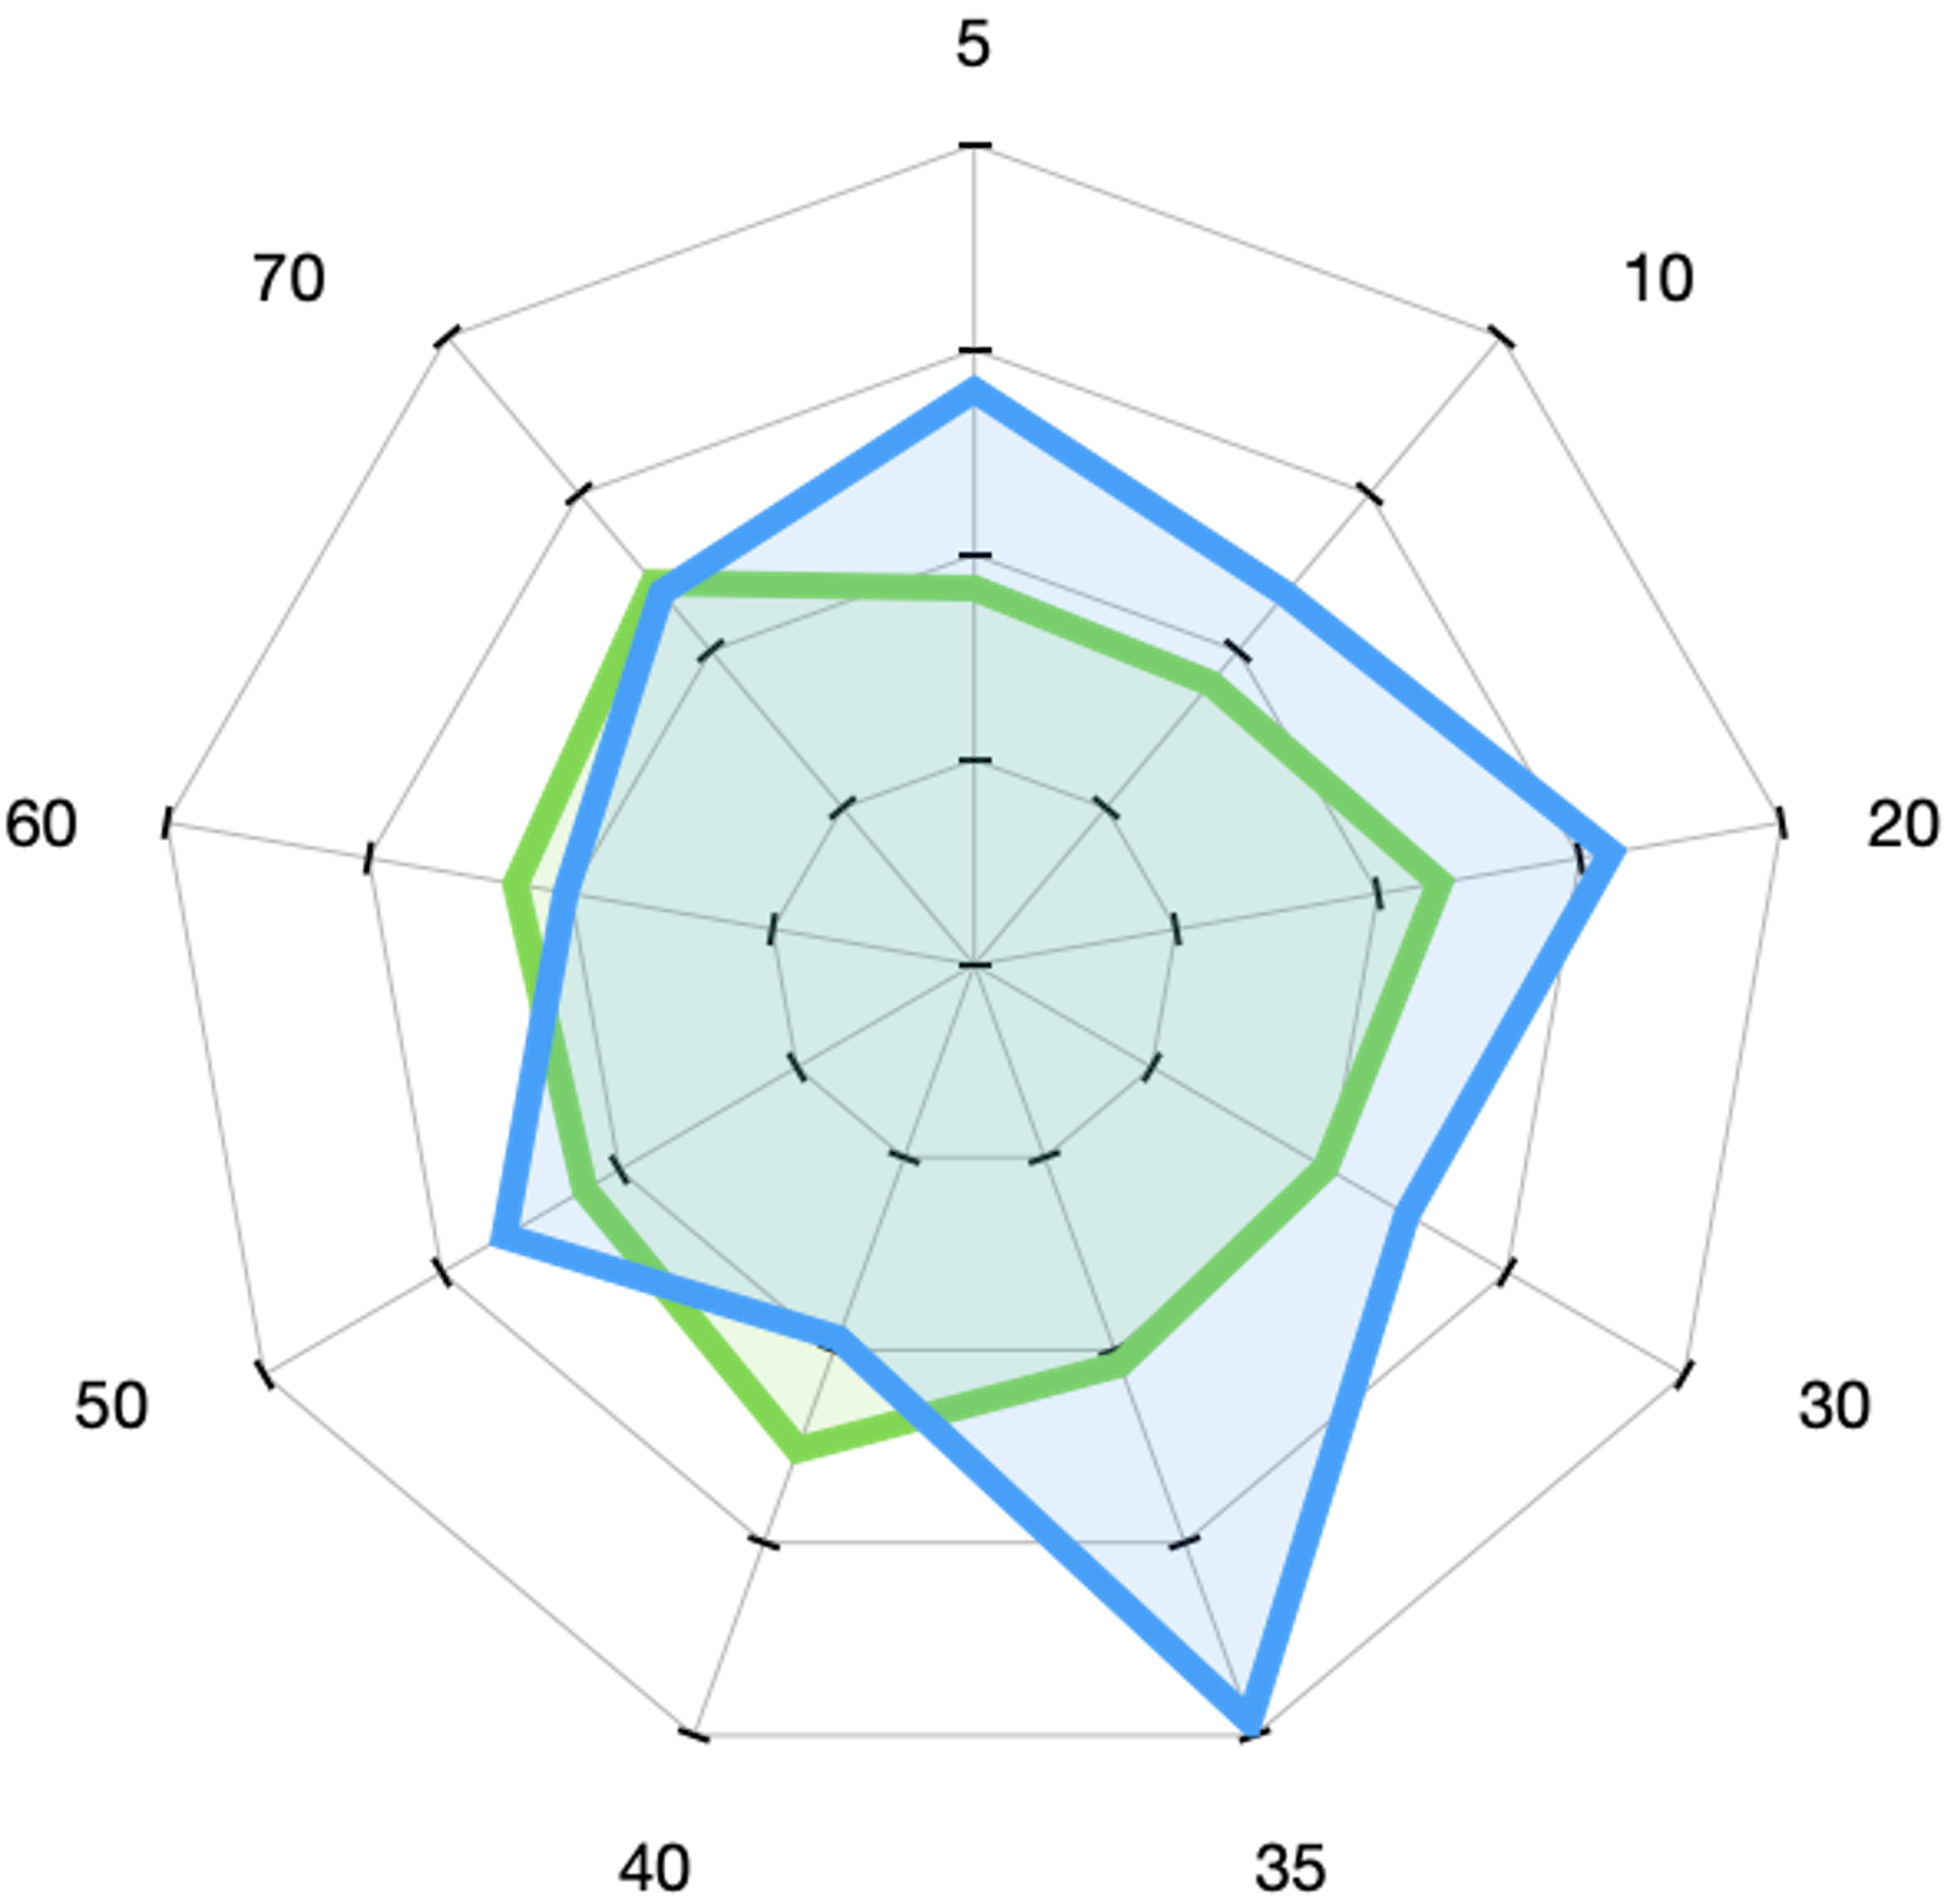
\includegraphics[scale=0.6]{GRU_RMSE_SPIDER.png}\label{fig:GRU_MAPE_SPIDER}}
\caption{Performance comparison of Upward batch and Downward batch ensemble(UD-Batch) and Corresponding upward and downward ensemble(CUD-ensemble) using DL models over MAPE performance measure.}
\label{fig:all_models_mape}
\end{figure}


\begin{table}[ht!]
\centering
\setlength{\tabcolsep}{3pt}
{\renewcommand{\arraystretch}{1}%
\caption{Performance of different DL models and proposed MBiS-DT models along \% improvement based on proposed MBiS-DT-Bi-LSTM }
\label{tab:Performance_of_different DL}
\begin{tabular}{p{0.1\textwidth}lllllllll}
\hline
\textbf{MODELS} & \textbf{MSE} & \textbf{\% Imp.} & \textbf{RMSE} & \textbf{\% Imp} & \textbf{MAE} & \textbf{\% Imp} & \textbf{MAPE} & \textbf{\% Imp} \\ \hline
LSTM & 1.97 &30.96\% & 1.39 &16.54\% & 1.07 &16.82\% & 4.33 &4.61\% \\
GRU & 3.35 &59.40\% & 1.78 &34.83\% & 1.45 & 38.62\% & 4.53 &8.83\% \\
BI-LSTM & 1.62 &16.04\% & 1.26 &7.93\% & 0.99 &10.10\% & 4.41 &6.34\% \\
RNN & 1.94 &29.89\% & 1.38 &15.94\% & 1.09 &18.34\% & 4.95&16.56\% \\
\textbf{Proposed MBiS-DT-LSTM} & \textbf{1.59} &14.46\% & \textbf{1.25} &7.20\% & \textbf{0.95} &6.31\% & \textbf{4.36} &5.27\% \\
\textbf{Proposed MBiS-DT-GRU} & \textbf{1.75} &22.28\% & \textbf{1.31} &11.45\% & \textbf{1.03} & 13.59\% & \textbf{4.26} &3.05\% \\
\textbf{Proposed MBiS-DT-RNN} & \textbf{1.52} &10.52\% & \textbf{1.23} &5.69\% & \textbf{0.97} &8.24\% & \textbf{4.55} &9.23\% \\
\textbf{Proposed MBiS-DT-Bi-LSTM} & \textbf{1.36} & - & \textbf{1.16} &- & \textbf{0.89} & - & \textbf{4.13} & - \\
\hline
\end{tabular}%
}
\end{table}


Table \ref{tab:Performance_of_different DL} provides a comparative analysis of experimented traditional models, namely LSTM, GRU, Bi-LSTM and RNN, and proposed models namely Proposed MBiS-DT-LSTM, Proposed MBiS-DT-GRU, Proposed MBiS-DT-RNN, Proposed MBiS-DT-Bi-LSTM based on key performance metrics, including MSE, RMSE, MAE and MAPE. The model Proposed MBiS-DT-Bi-LSTM is key performed over other traditional models and proposed models, so in terms of RMSE, the maximum improvement is 34.83\%, then GRU, and the minimum improvement is 5.69\%, then Proposed MBiS-DT-RNN. The MSE has maximum improvement, which is 59.40\%, then GRU and minimum improvement is 10.52\%, then Proposed MBiS-DT-RNN. Regarding MAE, the maximum improvement is 38.62\%, then GRU, and the minimum improvement is 8.24\%, then Proposed MBiS-DT-RNN. Regarding MAPE, the maximum improvement is 16.56\% then RNN, and the minimum improvement is 3.05\% then Proposed MBiS-DT-GRU. This comparative analysis concludes that the Proposed MBiS-DT-Bi-LSTM is the best performer model on various parameters like RMSE, MAE, MSE, etc,


% \begin{table}[ht!]
% \centering
% \subfloat{MAPE}
% \label{tab:MAPE}
% \begin{tabular}{lllll}
% \hline
% \textbf{MODELS} & \textbf{ORIGINAL} & \textbf{\% IMPROVEMENT} & \textbf{PROPOSED (P)} & \textbf{SHIFT LENGTH} \\ \hline
% \textbf{LSTM} & 4.33 & -7.78 & 4.36 & 20 \\
% \textbf{GRU} & 4.53 & 6.10 & 4.26 & 35 \\
% \textbf{BI-LSTM} & 4.41 & 6.31 & 4.13 & 35 \\
% \textbf{RNN} & 4.95 & 8.10 & 4.55 & 35 \\ \hline
% \end{tabular}
% \end{table}

% \begin{table}[ht!]
% \centering
% \subfloat{RMSE}
% \label{tab:RMSE}
% \begin{tabular}{lllll}
% \hline
% \textbf{MODELS} & \textbf{ORIGINAL} & \textbf{\% IMPROVEMENT} & \textbf{PROPOSED (P)} & \textbf{SHIFT LENGTH} \\ \hline
% \textbf{LSTM} & 1.39 & 10.0381 & 1.2593 & 20 \\
% \textbf{GRU} & 1.78 & 25.98 & 1.31 & 35 \\
% \textbf{BI-LSTM} & 1.26 & 7.99 & 1.16 & 35 \\
% \textbf{RNN} & 1.38 & 10.38 & 1.2343 & 35 \\ \hline
% \end{tabular}
% \end{table}
% \begin{table}[ht!]
% \centering
% \subfloat{MAE}
% \label{tab:MAE}
% \begin{tabular}{lllll}
% \hline
% \textbf{MODELS} & \textbf{ORIGINAL} & \textbf{\% IMPROVEMENT} & \textbf{PROPOSED (P)} & \textbf{SHIFT LENGTH} \\ \hline
% \textbf{LSTM} & 1.07 & 11.20 & 0.95 & 20 \\
% \textbf{GRU} & 1.45 & 28.8 & 1.03 & 35 \\
% \textbf{BI-LSTM} & 0.99 & 10.10 & 0.89 & 35 \\
% \textbf{RNN} & 1.09 & 11.24 & 0.97 & 35 \\ \hline
% \end{tabular}
% \end{table}



%\centering


\begin{figure}[!h]
\centering
\includegraphics[scale=0.23]{line_Plot.png}
\caption{Prediction plot of original test data(subset) corresponding to traditional DL models and proposed MBiS-DT $+$ DL's models.}
\label{fig:Line plot of vs proposed MBiS-DT models}
\end{figure}

In this line plot, Fig.\ref{fig:Line plot of vs proposed MBiS-DT models} of traditional models and proposed model prediction along with test data shows that our proposed models are closer to test data than traditional models. We have used the sub-part (40 data points.) test data for clear visualization. Overall, the line plot's results support the conclusion that the proposed models are better choices for temperature prediction than the traditional ones, making them valuable tools for meteorological forecasting and related applications. The outcome of this line plot is proposed that the MBiS-DT model line mimics better than traditional model lines on test data. So, the proposed MBiS-DT model is better than traditional models.

\begin{figure}[!h]
\centering
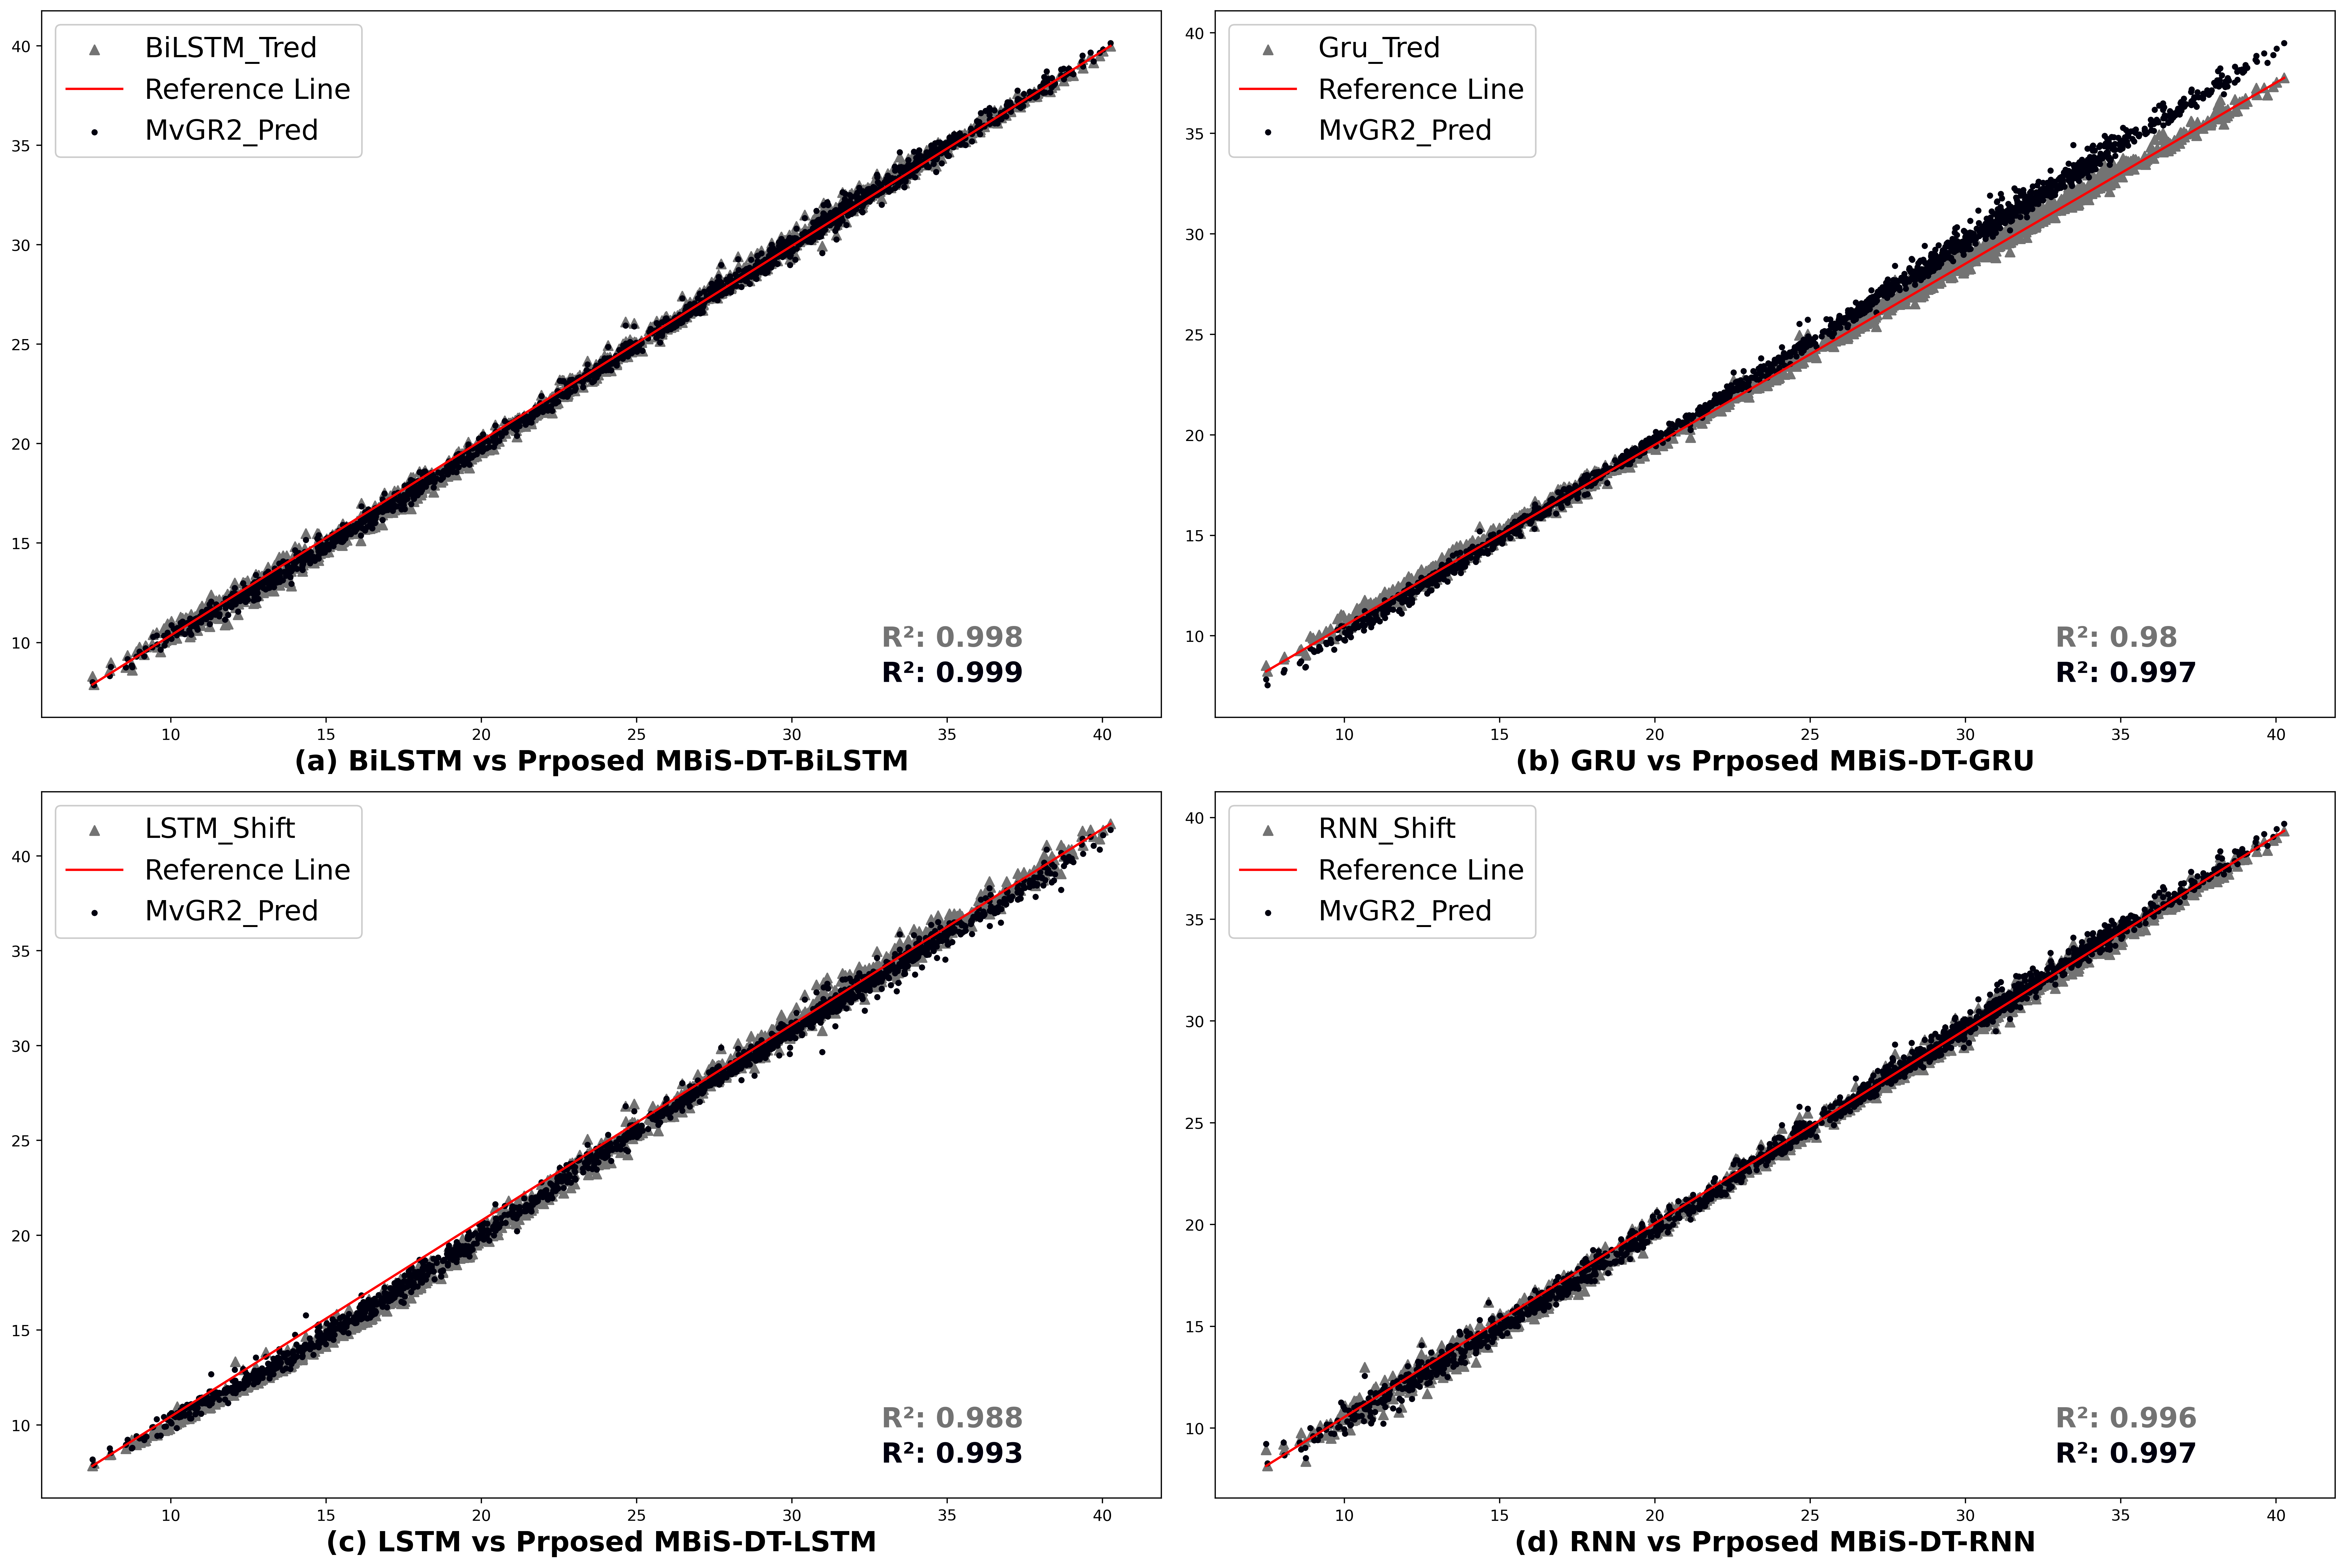
\includegraphics[scale=0.25]{scatter_Plot.png}
\caption{Superimposed prediction scattered plot of traditional DL and proposed model over test data.}
\label{fig:Scatter plot of vs proposed MBiS-DT models}
\end{figure}



In Fig.\ref{fig:Scatter plot of vs proposed MBiS-DT models}, the superimposed prediction scattered plot of traditional DL and proposed model over test data shows that the distribution of points is closest to the trend line. The $R^2$ values for RNN, GRU, BiLSTM, LSTM are 0.996, 0.98, 0.998, 0.988 respectively and values for Proposed MBiS-DT-RNN, Proposed MBiS-DT-GRU, Proposed MBiS-DT-LSTM Proposed MBiS-DT-Bi-LSTM are 0.997, 0.997, 0.993, 0.999. The more excellent value of $R^2$ shows the preciseness of data, so our proposed models have greater $R^2$ values than traditional models. This plot concludes that our proposed models are performing better than traditional models.



Table \ref{tabfri} presents a comprehensive analysis of various models used for temperature prediction based on multiple evaluation metrics, including MSE, RMSE, MAE, MAPE and their corresponding Friedman rankings. The proposed models outperform others, ranking all four at the top across all metrics. Proposed MBiS-DT-BiLSTM stands out as the best-performing model, ranking $ 1^{st}$ in all metrics, indicating superior accuracy, precision, and lower error rates. Collectively, in these proposed models, MBiS-DT-RNN achieves the lowest Friedman ranking of 3.5, signifying their exceptional performance. LSTM performs reasonably well, ranking $7^{th}$ in terms of MSE and RMSE, indicating moderate accuracy. It ranks $6^{th}$ in MAE and $3^{rd}$ in MAPE, showing that it's better at handling relative errors. It achieves a Friedman ranking of 5.75, which positions it in the middle of the pack. GRU ranks $8^{th}$ across all metrics, indicating relatively weaker performance than other models. It has the highest MSE, RMSE, MAE, and MAPE among the models evaluated, resulting in a Friedman ranking of 7.5, signifying its less favourable performance. BiLSTM performs consistently well, ranking $4^{th}$ across all metrics. It achieves relatively low MSE, RMSE, MAE, and MAPE values, indicating good accuracy and precision. With a Friedman ranking of 4.25, it is a competitive choice for temperature prediction. RNN ranks $6^{th}$ in MSE and RMSE, suggesting moderate accuracy. However, it ranks $7^{th}$ in MAE and $8^{th}$ in MAPE, indicating a higher relative error rate. Its overall performance is reflected in a Friedman ranking of 6.75. Also, in Fig.\ref{fig:FriedmanPic}, we shorted all models in ascending order of Friedman ranking for better visualization. Our proposed models are placed on starting indexes, which shows that our proposed models are better than other models. In conclusion, the table and figure demonstrate that the proposed models, remarkably Proposed Bi-LSTM, offer the most accurate and reliable temperature predictions compared to LSTM, GRU, BiLSTM, and RNN. These findings emphasize the potential of these models for enhancing meteorological forecasting and related applications. Table \ref{tabpvalue} presents a summary of p-values for statistical significance testing, with an alpha level of 0.05, comparing different pairs of algorithms used in the study. These p-values are crucial in assessing whether observed differences in model performance are statistically significant or merely due to random chance. Each row in the table compares two specific algorithms, with the p-value associated with that comparison. A small p-value, typically below 0.05, indicates that the difference in performance between the compared algorithms is statistically significant. Conversely, a larger p-value suggests that the observed differences could be due to random variability and are not statistically meaningful.
The first six rows reject the hypothesis. when $\alpha=0.05$. In essence, this table provides a concise summary of the statistical significance of performance differences between various algorithm pairs, aiding in interpreting the experimental results and identifying algorithms that demonstrate superior performance with statistical confidence.




%\section{This is an example for first level head---section head}\label{sec3}F
\begin{figure}[ht!]
\centering
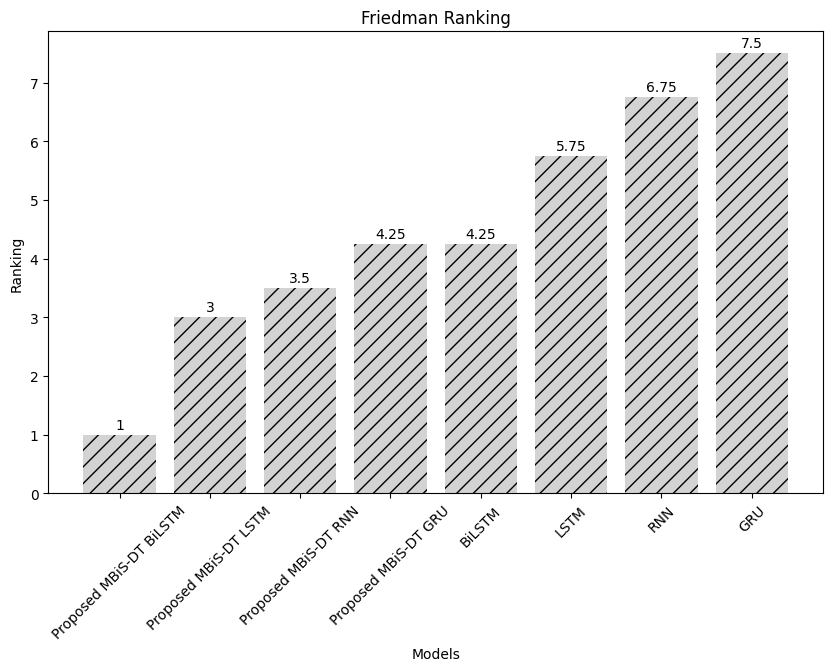
\includegraphics[width=0.9\textwidth, height=0.6\linewidth]{freidman_rank.png}
\caption{Aggregated Friedman ranking of proposed (MBiS-DT) models and traditional models over RMSE, MAE, MSE and MAPE.}
\label{fig:FriedmanPic}
\end{figure}

\begin{table}[ht!]

    \setlength{\tabcolsep}{3pt}
    {\renewcommand{\arraystretch}{1}%
\caption{ranking of different models based on performance measures}
\label{tabfri}
\begin{tabular}{l|lllll}
\hline
\\
Models& MSE & RMSE & MAE & MAPE & Friedman ranking\\
\hline
\\
LSTM & 7 & 7 & 6 & 3 & 5.75 \\
GRU & 8 & 8 & 8 & 6 &7.5 \\
BiLSTM & 4 & 4 & 4 & 5 &4.25 \\
RNN & 6 & 6 & 7 & 8 &6.75 \\
Proposed MBiS-DT-LSTM & 3 & 3 & 2 & 4 & 3 \\
Proposed MBiS-DT-GRU & 5 & 5 & 5 & 2 &4.25 \\
Proposed MBiS-DT-RNN & 2 & 2 & 3 & 7 &3.5 \\
Proposed MBiS-DT-Bi-LSTM & 1 & 1 & 1 & 1 &1 \\ \hline
\end{tabular}%
    }

\end{table}


%\begin{table}[!htp]
%\centering
%\begin{tabular}{|c|c|}\hline
%Algorithm&Ranking\\\hline
%LSTM & 5.75\\
%GRU & 7.5\\
%BiLSTM & 4.25\\
%RNN & 6.75\\
%Proposed LSTM & 3\\
%Proposed GRU & 4.25\\
%Proposed BiLSTM & 1\\
%Proposed RNN & 3.5\\
%\hline
%\end{tabular}
%\subfloat{Average Rankings of the algorithms}
%\label{tab:Friedman}
%\end{table}
Adjusted p-values for $\alpha$=0.05 is represented in Table \ref{tabpvalue}
%\begin{table}[!htp]
%\centering\scriptsize
%\begin{tabular}{cccc}
%$i$&algorithms&$z=(R_0 - R_i)/SE$&$p$\\
%\hline6&GRU vs. BiLSTM&2.738613&\textbf{0.00617\\
%5&LSTM vs. BiLSTM&1.917029&0.055234\\
%4&BiLSTM vs. RNN&1.917029&0.055234\\
%3&LSTM vs. GRU&0.821584&0.411314\\
%2&GRU vs. RNN&0.821584&0.411314\\
%1&LSTM vs. RNN&0&1\\
%\hline
%\end{tabular}
%\subfloat{P-values Table for $\alpha=0.05$}
%\label{tab:pvalue}
%\end{table}

\begin{table}[!htbp]
\centering\scriptsize
    \setlength{\tabcolsep}{3pt}
    {\renewcommand{\arraystretch}{1}%

\caption{Pair-wise p-values of traditional and proposed DL models with z-score and p-value($\alpha=0.05$)}
\label{tabpvalue}
\begin{tabular}{cccc}
\hline
$i$&algorithms&$z=(R_0 - R_i)/SE$&$p$\\
\hline28&GRU vs. Proposed MBiS-DT-Bi-LSTM&3.752777&\textbf{0.000175}\\
27&RNN vs. Proposed MBiS-DT-Bi-LSTM&3.319764&\textbf{0.000901}\\
26&LSTM vs. Proposed MBiS-DT-Bi-LSTM&2.742414&\textbf{0.006099}\\
25&GRU vs. Proposed MBiS-DT-LSTM&2.598076&\textbf{0.009375}\\
24&GRU vs. Proposed MBiS-DT-RNN&2.309401&\textbf{0.020921}\\
23&RNN vs. Proposed MBiS-DT-LSTM&2.165064&\textbf{0.030383}\\
22&GRU vs. Bi-LSTM&1.876388&0.060602\\
21&GRU vs. Proposed MBiS-DT-GRU&1.876388&0.060602\\
20&Bi-LSTM vs. Proposed MBiS-DT-BiLSTM&1.876388&0.060602\\
19&RNN vs. Proposed MBiS-DT-RNN&1.876388&0.060602\\
18&Proposed MBiS-DT-GRU vs. Proposed MBiS-DT-Bi-LSTM&1.876388&0.060602\\
17&LSTM vs. Proposed MBiS-DT-LSTM&1.587713&0.112351\\
16&Bi-LSTM vs. RNN&1.443376&0.148915\\
15&RNN vs. Proposed MBiS-DT-GRU&1.443376&0.148915\\
14&Proposed MBiS-DT-Bi-LSTM vs. Proposed MBiS-DT-RNN&1.443376&0.148915\\
13&LSTM vs. Proposed MBiS-DT-RNN&1.299038&0.193931\\
12&Proposed MBiS-DT-LSTM vs. Proposed MBiS-DT-Bi-LSTM&1.154701&0.248213\\
11&LSTM vs. GRU&1.010363&0.312321\\
10&LSTM vs. Bi-LSTM&0.866025&0.386476\\
9&LSTM vs. Proposed MBiS-DT-GRU&0.866025&0.386476\\
8&Bi-LSTM vs. Proposed MBiS-DT-LSTM&0.721688&0.470486\\
7&Proposed MBiS-DT-LSTM vs. Proposed MBiS-DT-GRU&0.721688&0.470486\\
6&LSTM vs. RNN&0.57735&0.563703\\
5&GRU vs. RNN&0.433013&0.665006\\
4&BiLSTM vs. Proposed MBiS-DT-RNN&0.433013&0.665006\\
3&Proposed MBiS-DT-GRU vs. Proposed MBiS-DT-RNN&0.433013&0.665006\\
2&Proposed MBiS-DT-LSTM vs. Proposed MBiS-DT-RNN&0.288675&0.77283\\
1&Bi-LSTM vs. Proposed MBiS-DT-GRU&0&1\\
\hline
\end{tabular}%
}
\end{table}
\pagebreak
